%====================== header ==================================================
\documentclass[12pt]{osuthesis}

\usepackage{listings}

\usepackage{color}
% \usepackage[table,xcdraw]{xcolor}
\usepackage{lscape}


\definecolor{codegreen}{rgb}{0,0.6,0}
\definecolor{codegray}{rgb}{0.5,0.5,0.5}
\definecolor{codepurple}{rgb}{0.58,0,0.82}
\definecolor{backcolour}{rgb}{0.95,0.95,0.92}

\lstdefinestyle{mystyle}{
	backgroundcolor=\color{backcolour},   
	commentstyle=\color{codegreen},
	keywordstyle=\color{magenta},
	numberstyle=\tiny\color{codegray},
	stringstyle=\color{codepurple},
	basicstyle=\footnotesize,
	breakatwhitespace=false,         
	breaklines=true,                 
	captionpos=b,                    
	keepspaces=true,                 
	numbers=left,                    
	numbersep=5pt,                  
	showspaces=false,                
	showstringspaces=false,
	showtabs=false,                  
	tabsize=2
}

\lstset{style=mystyle}

%====================== process the document configuration ======================
%====================== font dependent settings
\renewcommand{\labelitemi}{$\bullet$}

%====================== provides some shapes, not necessarily used directly =====
\usepackage{pict2e}

%====================== get rid of tiny overfull box warnings ===================
\hfuzz=3pt

%====================== create an execute function so we can shell out ==========
\def\execute{%
    \begingroup
    \catcode`\%=12
    \catcode`\\=12
    \executeaux}
\def\executeaux#1{\immediate\write18{#1}\endgroup}

%====================== indexing ================================================
\usepackage{makeidx} %index package
\execute{makeindex main}
\makeindex

%====================== nomenclature ============================================
\usepackage{nomencl}
% nomenclature subgroup syntax
% B = subscript
% P = superscript
% R = roman symbols
% G = greek symbols
%originally we had the nomgroup redefinition here, but it needs to be in the same
%  document as the printnomenclature command...or so it seems
%convert the .nlo list into the proper nomenclature
% environment in .nls by using style nomencl.ist
\execute{makeindex main.nlo -s nomencl.ist -o main.nls}
\makenomenclature

%====================== bibliography ============================================
% OLD DEFAULT CLASS
%\usepackage[super]{natbib} %bibliography citation style with round brackets

\usepackage{cite}

%====================== AMS math packages =======================================
\usepackage{amsmath}
\usepackage{amsxtra}
\usepackage{amstext}
\usepackage{amssymb}

%====================== Tables, figures =========================================
\usepackage{array}
\usepackage{subfig}
\usepackage{rotating}

%====================== Units package ===========================================
\usepackage[squaren]{SIunits}

%====================== Other packages ==========================================
\usepackage{graphicx} %convenient graphics import package
\usepackage{ifthen}       %Add ifthenelse support
\usepackage{enumerate} %modify enumerate style
\usepackage[usenames,dvipsnames]{xcolor}
\usepackage[colorlinks,citecolor=Black,linkcolor=Black,urlcolor=Black,filecolor=Black]{hyperref}
\usepackage{url} % allow typsetting urls
\usepackage{setspace} % allow easy variation of line spacing
\usepackage{lipsum}

%====================== margin comments ========================================
\setlength{\marginparwidth}{1.0in}
\setlength{\marginparsep}{0.1in}
\let\oldmarginpar\marginpar
\renewcommand\marginpar[1]{\-\oldmarginpar[\raggedleft\tiny #1]{\raggedright\scriptsize\color{red} #1}}

%============ tell LaTeX where to find images ===================================
\graphicspath{
              {Ch-Introduction/images/}
              {Ch-IceXI/images/}
              {Ch-ConformerLandscapes/images/}
              {Ch-Germanium/images/}
              {Ch-2dWater/images/}
              {Ch-Conclusion/images/}
             }

%============ specify how deep layout numbering goes ============================
\setcounter{secnumdepth}{3} %3 specifies to number down to subsection
\setcounter{tocdepth}{3} %3 specifies to include down to subsections in the TOC




%====================== read any new commands or environments ===================
%% User defined commands here

\newcommand{\RB}[1]{\left[#1\right]}
\newcommand{\PB}[1]{\left(#1\right)}
\newcommand{\SB}[1]{\left|#1\right|}
\newcommand{\CB}[1]{\left\{#1\right\}}

%\let\origitemize\itemize
%\renewenvironment{itemize}{\origitemize\setlength{\itemsep}{1pt}\setlength{\parskip}{0pt}\setlength{\parsep}{0pt}}{\endlist}
%
%\let\origdescription\description
%\renewenvironment{description}{\origdescription\setlength{\itemsep}{1pt}\setlength{\parskip}{0pt}\setlength{\parsep}{0pt}}{\endlist}
%
%\let\origenumerate\enumerate
%\renewenvironment{enumerate}{\origenumerate\setlength{\itemsep}{1pt}\setlength{\parskip}{0pt}\setlength{\parsep}{0pt}}{\endlist}
%
%\newenvironment{chapterAbstract}
%    { %before environment contents...
%      \begin{quote}
%        \begin{flushleft}
%            \begin{Large} Abstract \end{Large}
%        \end{flushleft}
%        \vspace{-1em}
%        \hrulefill
%        \vspace{-1.7em}
%        \begin{singlespacing}
%    }
%    { %after environment contents...
%         \end{singlespacing}
%        \vspace{-1em}
%        %\hrulefill
%      \end{quote}
%    }
%
\newenvironment{dedication}
   {\vspace{6ex}\begin{quotation}\begin{center}\begin{em}}
   {\par\end{em}\end{center}\end{quotation}}

%====================== document information ====================================
\title{EXPLORING CRITICAL CONFORMATIONS}

\formattedtitle{EXPLORING CRITICAL CONFORMATIONS: \\ STATE SEARCHING AND SAMPLING IN\\BOTH GERMANIUM CHAINS AND ICE}

\author{GENTRY H. SMITH}

\degreeone{\\ B.S. \\
        Southern Nazarene University\\
        Bethany, OK, USA\\
        2016}

\degreesought{Master of Science}

\degreedate{December 2018}

\majorfield{Chemistry}


\begin{document}

%====================== make title page =========================================
\maketitle

%====================== make approval page ======================================
\makeapproval{3} % use this for the page your committee will sign
%\makeElectronicapproval{4} % use this page for the electronic thesis submission

%====================== make acknowledgments page ===============================
\begin{acknowledge}
	\begin{acknowledge}

To Oklahoma State University, for providing the environment in which I have been able to study, teach, and research.

To the HPCC and the individuals within \textbf{(get first/last names)} for providing a powerful cluster for computations and continuous support for technical issues.

To my advisor, who instructed and assisted me in research

To my parents, by blood and marriage, who have always encouraged me toward higher goals.

To my wife, Miranda, who has supported me for over 5 years. 

%    \clearpage
%    \vspace{3in}
%    \begin{dedication}
%    You can do this. \\ ---Caffeine
%    \end{dedication}

\end{acknowledge}

\end{acknowledge}

%====================== make abstract ===========================================
\renewcommand{\thepage}{\roman{page}}
\begin{abstract}{GENTRY H SMITH}{JUNE, 2018}{COMPUTATIONAL CHEMISTRY}
    Molecular conformation plays a critical role in the properties of systems in both the condensed or vapor states. 
The ensemble of conformations dictates structural properties, average energy, heat capacities, and other thermodynamic and dynamic quantities. 
Here, we explore the role of conformation in proton ordering and orientational defect formation in ice as well as strategies for exhaustive conformer searching for molecules using Group IV element backbones. 
In the ice systems, we show algorithmic strategies for seeking optimized proton disordered crystals that satisfy the Bernal-Fowler ice rules. 
In the Group IV molecule investigations, we develop an automated strategy for seeking the optimal low energy conformer and uncover previously unreported deficiencies in common computational software used in investigating Germanium complex energies.
\end{abstract}

%====================== table of contents creation ==============================
\tableofcontents

%====================== table of tables creation ================================
\listoftables

%====================== list of figures creation ================================
\listoffigures

%====================== nomenclature ============================================

%====================== nomenclature -- must be customized here ===================
% ==== Redefine the command called for sorting the nomenclature
\renewcommand{\nomgroup}[1]
    {%
     \ifthenelse{\equal{#1}{A}}{\vspace{0.3cm}\item[\textbf{Variables}]}{
      \ifthenelse{\equal{#1}{G}}{\vspace{0.3cm}\item[\textbf{Greek Symbols}]}{
       \ifthenelse{\equal{#1}{B}}{\vspace{0.3cm}\item[\textbf{Subscripts/Superscripts}]}{
       }
      }
     }
    }
% ==== Redefine the length between items in the nomenclature
\setlength{\nomitemsep}{-\parsep}
% ==== Redefine the page to be roman numerals
\renewcommand{\thepage}{\roman{page}}
% ==== Set the value of page to the value of placeholder...which is apparently
%      passed from the previous environment
\setcounter{page}{\value{placeholder}}
% ==== Redefine the nomenclature name to be more inline with other dissertation environments
\renewcommand{\nomname}{\centering \ssp \rule{0in}{1in} \par
    NOMENCLATURE \par
    \vspace*{0.25in} \par \dsp}
% ==== Add a preamble statement to the nomenclature
%\renewcommand{\nompreamble}{The following is a list of symbols, variables, and scripts used in this work which may not be defined as they are encountered in the body.}
% ==== Redefine the nomenclature label to have trailing dots filling up the box
\renewcommand{\nomlabel}[1]{#1\nobreakspace\dotfill}
% ==== Print the nomenclature to the pdf
{\ssp \printnomenclature[0.75in]}

\nomenclature[aV ]{$V$}{Lennard-Jones Potential intermolecular potential }
\nomenclature[aS ]{$\sigma$}{Lennard-Jones Potential intermolecular contact distance}
\nomenclature[aE ]{$\epsilon$}{Lennard-Jones Potential well depth}
\nomenclature[ar ]{$r$}{Lennard-Jones Potential distance between center of two particles}
%\nomenclature[aGr]{$G_r$}{Net radiation into the surface}
%\nomenclature[aN ]{$N$}{Number or count of a material or property}

%\nomenclature[g1 ]{$\alpha$}{Thermal diffusivity}
%\nomenclature[g3 ]{$\gamma$}{Psychrometric constant}

\nomenclature[b0 ]{$0$}{Initial condition}
%\nomenclature[ba ]{$a$}{Property of the air}
%\nomenclature[bc ]{$c$}{Radial centroid}



%====================== main  body of the dissertation ==========================
% ==== Get a new page to leave the last page of the nomenclature unaffected
\newpage
% ==== Set line spacing for the bulk of the document
%\setstretch{1.4}
\doublespacing
% ==== Reset page numbering to arabic numerals...this also resets it to start at 1
\pagenumbering{arabic}


%====================== chapters information ====================================
\chapter{Introduction}
\label{ch:Introduction}

\section{Computational Chemistry: Chemistry on the Computer}

For nearly a century, computational methods have greatly assisted chemists in their efforts of research and discovery.
% EXAMPLES? CITATION NEEEDED
As a standalone field, computational chemistry uses computer simulations to solve chemical problems. 
These simulations typically rely on theoretical methods adapted to run highly efficiently on computers.
While initial computational methods were designed to solve wave functions and atomic orbitals, the scope quickly expanded into multiple fields of chemistry as more methods were developed to confirm or predict properties of molecules and systems.
%With the introduction of \textit{ab initio} and density functional methods, computational methods began to stand as a distinct field within chemistry. 
This introduction serves to introduce necessary background information generally relevant to the methods developed and utilized in the following chapters.

\section{Relevant Computational Methods}

%REBUILD
%Analytical descriptions of molecular systems are ideal because 
%...
%however
%...
%so we use numerical approaches
%...

Modern computational methods take one of several approaches in computing a system.
Usually limited by the scale of molecule and scope of system, multiple methods exist to analytically solve or closely approximate a system by way of solving or approximating the quantum mechanical wave function or through a similarly consistent method of generalization by way of statistical solutions.
Many other methods exist, but are not directly relevant to this work.

The first hurdle in any computational system is the likely impossibility of analytically solving the problem. 
In a system with more than two particles, this multi-body problem usually cannot be solved analytically excepting the dihydrogen cation due to the electron-electron correlation term being situationally dependent.
%This is largely due to the complexity introduced into the wave function of multiple interacting species that often lead to prohibitively large or impossible equations to solve.

\subsection{Quantum Mechanical Methods and Basis Sets}

In computational chemistry, quantum mechanical methods generally refer to computational methods that attempt to solve, or closely approximate, the electronic Schr\"{o}dinger equation given nuclei and electron position information to determine properties of the system like energies or electron densities.
Because the Schr\"{o}dinger equation is impossible to solve exactly for many-body systems, different methods use different approximations to balance between accuracy of the approximation and efficiency of computation.

\subsubsection{\textit{Ab Initio} Methods}

\textit{Ab initio}, or ``from first principles," methods refer to calculation methods that rely solely on physical constants as external values.
By design, \textit{ab initio} methods avoid using any empirically-acquired data and rely on theoretically calculated values.
The development of these methods allowed computational chemists to solve a new class of problems and resulted in John Pople and Walter Kohn receiving the Nobel Prize in Chemistry in 1998 for their work.
The \textit{ab initio} method utilized in this work is the Hartree-Fock (HF) method used to determine the energy of a many-body system in a stationary state, which is to say time-independent.\cite{hartree_1928}
Known initially as the self-consistent field method, the HF method utilizes approximations defined by the basis set to approximate the Schr\"{o}dinger equation. 
The consistency of this self-consistent field method arose by the requirement that the final calculated field be self-consistent with the initial field.
An additional property of HF is that electron-electron repulsion is not taken into account, requiring that a basis set account for this interaction.
As larger basis sets are used, the overall energy of the wavefunction is decreased toward a value known as the Hartree-Fock limit.
This limit is approached as the larger basis sets approach the exact solution of the non-relativistic Schr\"{o}dinger equation without spin orbital terms.
The calculation of relativistic and spin terms require a further method known as Post-Hartree-Fock, which is not used considered further in this work.

\subsubsection{Density Functional Theory Methods}

Density Function Theory (DFT) Methods function very similarly to \textit{ab initio} methods in how Slater-type orbitals are used to approximate the Schr\"{o}dinger equation, but differ in that DFT utilizes some empirical data to speed up the calculation process.\cite{DFT}
These simplifications are able to model exchange and correlation interactions very well, however the reliability of calculated properties, specifically intermolecular interactions, dispersion forces, and other internal properties are greatly reduced.
Just as with \textit{ab initio} methods, DFT methods require a basis set definition for the approximation calculations.
Many DFT methods exist and even some so-called hybrid functional methods that exchange with HF terms for greater reliability in calculated values.
One pure DFT method used in this work is BLYP, which utilizes  the Becke exchange with the Lee-Yang-Parr correlation part.
Some hybrid functional methods used are the B3LYP, M06L, and PBE methods.
The B3LYP utilizes the BLYP but combined Becke's exchange with the exact energy from HF theory.
M06L, known as the Minnesota functionals, depend on kinetic energy density values from databases.
It specifically was designed to work well with transition metals, inorganics, and organometallics.\cite{M06L}
The PBE method, developed by Perdew, Burke, and Ernzerhof,  is another method with similar levels of accuracy to B3LYP that attempts to increase the number of HF-exchanged functionals.\cite{PBE}

\subsubsection{Semi-Empirical Methods}

Like DFT, semi-empirical methods also pull somewhat from Hartree-Fock methods, but rely even more on approximations and empirical data to nearly completely substitute out any proper calculation of the Schr\"{o}dinger equation.
These data can produce fairly accurate results to experimental data, but rely heavily on a similarity between the subject molecule and the database molecules.
Due to its restrictive scope, semi-empirical methods excel in organic chemistry calculations where relatively few elements are used with systems with hundreds of atoms.\cite{huckel}
% ^^^ WE SURE BOUT THAT?
Additionally, various semi-empirical methods have been designed to produce results with close accuracies to specific sets of experimental data.
Two methods used in this work, AM1\cite{AM1} and PM3,\cite{PM3} reproduce well heats of formation, dipole moments, ionization potentials, and structural geometries.
Unlike the other methods described so far, basis sets are not used at all in the calculation of energies and properties.

\subsubsection{Basis Sets}

While running calculations, both \textit{ab initio} and DFT methods require basis sets to represent the electronic wave function as a system of algebraic equations that can be efficiently calculated.
While basis sets can be designed with atomic orbitals or plane waves, this work focus primarily on basis sets designed with atomic orbitals.
The two most often used types of orbitals are Gaussian-type and Slater-type orbitals.
Slater-type orbitals (STOs), named after the physicist John Slater who introduced them in 1930,\cite{SlaterOrbitals} function as a linear combination of atomic orbitals (LCAO) adopted as a molecular orbital. 
STOs notably exhibit similar features as Schr\"{o}dinger-based orbitals, excepting that STOs have no radial nodes.

Gaussian-type orbitals (GTOs), introduced by S. Francis Boys in 1950,\cite{GaussianOrbitals} also function as orbitals in the LCAO method.
GTOs are similar to STOs in premise, but have further reduced realism when compared to Schr\"{o}dinger-based orbitals.
One example of this is the lack of accuracy of electron density near the nucleus.
While exhibiting a lesser accuracy, GTOs excel in computational efficiency compared to STOs by roughly 4-5 orders of magnitude.
This allows GTO-based calculations to compute more orbitals.
Specifically, Boys designed GTOs as a method of approximating STOs.

Basis sets are often grouped by their sizes.
The smallest sets, known as minimal basis sets, use a single basis function for each orbital. 
The most common minimal basis set, STO-nG where n is an integer usually between 2 and 6, was first proposed by John Pople in 1969.\cite{PopleSTO}
This method describes that a Slater-type orbital can be approximated using n Gaussian orbitals.
These STO-nG approximations end up fitting electron densities well at all radial distances except those close to the nucleus.
The STO-3G basis set used in this work is a popular basis set as the 3 Gaussian-type orbitals approximation works well for atoms in the [H-Xe] range.

The other basis sets used in the work fall under the category of split-valence basis sets.
These basis sets represent valence electrons with more than one basis function, which allows for electron density to be more flexible in different molecular systems.
The most common form of these basis sets was introduced by John Pople as the X-YZg form and are commonly referred to as Pople basis sets.\cite{PopleBS}
These follow the form that each orbital basis function is comprised of X Gaussians.
The Y and Z represent an additional linear combination of Gaussian functions made of Y and Z Gaussians  that compose the valence. 
These basis sets are not limited to two valence functions, referred to as a double-zeta, and can also be triple- or quadruple-zeta.
Additional values, typically denoted by one or two stars, one or two plus signs, or explitly-defined orbital combinations in parentheses can also be used to further expand the basis set as desired.
The star notation defines a polarization function for heavy atoms to account for d and f polarizations.
The plus signs denote diffuse functions that more-accurately represent less common valence electrons like carbanions that may diffuse further out from the nucleus.

\subsection{Monte Carlo Molecular Modeling}

As systems increase, approximations quickly approach infeasibly-high calculation times.
A method of working around this problem is known as Monte Carlo methods, or MC.
While not named until the 1950s, MC methods were first seen in the 18$^{th}$ century thought experiment Buffon's needle.\cite{buffon}
In his work, Buffon proposed dropping $n$ needles of length $l$ onto a plane with parallel lines spaced $t$ units apart.
Buffon worked out that the probability, $P$, of a needle crossing one of the lines to be $P=\frac{2l}{t\pi}$.
Solving for $\pi$, the probability can be rearranged as $\pi=\frac{2l}{tP}$ to approximate $\pi$.
Since $P$ can also be approximated by dividing the number of needles crossing one the of the lines, $h$, by the $n$ needles as $P=\frac{h}{n}$, the approximation can be expressed as $\pi=\frac{2l*n}{th}$.

This method of randomness was improved upon by Stanislaw Ulam while working at Los Alamos National Laboratory in the late 1940s by introducing Markov chains to favor the probability of events occurring.
Ulam shared this work with John von Neumann and together they created a program to run on the Electronic Numerical Integrator and Computer (ENIAC) capable of computing this favored version of random sampling.
As the project was secretive due to being used as a part of the Manhattan Project, a collaborator named Nikolas Metropolis suggested the name Monte Carlo due to Ulam's uncle's propensity to gambling at a casino in Monaco of the same name.\cite{MCOrigins}
Later dubbed Markov Chain Monte Carlo (MCMC) sampling, this allowed for random sampling to instead become a virtual statistically-appropriate sampling method.
Eventually published in 1949 by Metropolis and Ulam, this laid the groundwork for MC methods used in modern chemical simulation packages. 


\section{Hardware}

Since computation methods were developed slightly before and during the rise of modern computers, early calculations were performed by hand with minimal assistance by machines. 
Over time, these methods were increasingly assisted by early computers and further development eventually led to the first computational programs.
These first computers, like the ENIAC and its successor Electronic Discrete Variable Automatic Computer (EDVAC) offered computation power in the order of a few dozen to a few thousand operations per second.

For this work, the majority of calculations were computed on the Oklahoma State University Cowboy Cluster. 
Available since 2012, this cluster collectively offers the computing power of 3048 cores and 8576 GB of RAM, totaling 48.8 trillion FLoating point Operations Per Second (Tera FLOPS or TFLOPS). 

\section{Software}

If hardware denotes the realm of study of a computational chemist, software denotes the tools. 
By utilizing preexisting packages and developing new and more advanced tools, computational chemists are able to simulate a wide variety of chemical systems.

\subsection{Programs}

While chemical computational programs have existed for nearly 50 years, additional programs have relatively recently developed to aid in the visualization and depiction of chemical systems.
Gaussian, developed by John Pople and his team, was the first popular \textit{ab initio} computation program.
Released as Gaussian 70 in 1970, it has received regular updates and capability expansions, and is one of the most widely-used computational chemistry tools available in its latest iteration, Gaussian 16.
Gaussian tends to carry a lot of clout in the computational community as founder John Pople won a Nobel Prize in 1998 with Walter Kohn for his work in \textit{ab initio} quantum mechanical systems and for being one of the oldest packages around.

In addition to Gaussian, many other chemical computational packages exist.
Two additional packages used in this work are GAMESS,\cite{GAMESS} a package also in active development since the 1970s led by Mark Gordon, and NWChem,\cite{NWChem} a popular open source package developed by Pacific Northwest National Laboratory since the late 2000s.

Once a set of calculations has completed, investigators often report the calculated system graphically through visualization tools.
These tools are also popular among any investigator wishing to represent a compound or system as more than its molecular formula.
Two visualization tools used in this work are Avogadro and UCSF Chimera.
Avogadro, in development since 2008, is a relatively simple molecular visualization tool designed to work across multiple operating systems.\cite{Avogadro}
UCSF Chimera, developed by the Resource for Biocomputing, Visualization, and Informatics (RBVI) at the University of California, San Francisco, focuses on more advanced representations of compounds and systems. It allows for multi-structure files to generate videos of simulations and also provides a powerful Application Program Interface for programmatically creating or altering molecules and systems.\cite{UCSFChimera}

\subsection{Programming Languages}

A final note should be made about programming languages and their usage in general and in this work.
Programming languages have existed for as long as computers.
From original punch cards and bitwise commands to modern interpreted languages, programming languages allow investigators to control computers to enact explicit commands.
In a way, the job command files in computational tools like those in Gaussian and GAMESS are programmatically used as a programming language to tell a system to enact a calculation of type X on system Y with Z parameters.
Even these tools utilize code to enact their commands, usually in older and highly efficient languages like C and Fortran that are compiled into machine code.
Because these tools directly interact with hardware to complete an immense number of calculations, efficiency is key.

One language almost exclusively used in this work is Python.\cite{Python} 
The Python programming language has recently become one of the most used programming languages for scientific analysis.
This is possibly due to Python's initial development focus of data analysis, support for extensions by the development team, and ease of use.
As a scripted type language, Python is not compiled for specific hardware like code written in C and Fortran languages, but certain packages and extensions can take advantage of those efficiency boosts to improve Python's effectiveness.
Math and science packages like NumPy\cite{NumPy} and SciPy\cite{SciPy} interface with C code to rapidly speed up complex mathematic evaluations like matrix manipulations while retaining the usability expected in Python.
Additional packages like Cython\cite{Cython} will take a completed Python script and compile much of it in C code to greatly improve efficiency and reduce the computational strain on the system.

As will be seen in this work, code can be used to generate and run these sets of code, effectively creating a train of code that can operate as a tool within a tool. 
One aspect of this is abstracting out methods and basis sets to that of a computational requirement and level of accuracy.
% THIS IS WEIRD. FIX ,,,
%Effectively, an investigator could remove any necessary knowledge of which basis set or method is necessary for a specific system, although a tool with sufficient awareness to automatically enact this has not been published.















\chapter{On Algorithms for Building and Sampling Disordered Crystal States}
\label{ch:iceXI}

\section{States and Properties of Ice}

Ice is cool. 
Ice has many forms, each with unique environments and structures that give rise to similar and unique properties. 

\subsection{Bernal-Fowler Ice Rules}

Bernal-Fowler Ice Rules are the basic rules for how water molecules interact in an ice structure.
DETAILS ON BF PAPER

Basically, water's tetrahedral structure allows for four interactions on each molecule. 
The two protons allow for a hydrogen bond with a lone pair from a neighboring oxygen atom.
Similarly, the oxygen atom's two lone pairs allow for a hydrogen bond with a neighboring proton. 
These rules are fairly rigid in the sense that every water molecule can interact with two oxygen atoms and two protons from four surrounding water molecules.
These are also free-form in the sense that each of the four attached water molecules can occupy one of three rotational microstates, allowing for 81 possible configurations (including rotational duplicates).

\subsection{Forms of Ice}

While ubiquitous in the 'I$_{h}$' form, ice water has many known forms.
As of the writing of this work, there are 17 established forms of ice. 
These forms usually occur in cubic, hexagonal, and orthorhombic crystal structures.
The relationship between external pressure and temperature are the primary defining characteristics of which form will form in a given system. 
Do other characteristics come into play??????? %FIND OUT


\subsection{Ice I$_{h}$}

As the most commonly found form on earth, ice I$_{h}$ is a highly desired form for computational studies involving ice systems. 
%structure
%P/T deets
As an interesting specificity, ice I$_{h}$ does not cover any proton-disordered crystal with the same oxygen spatial positioning. 
Rather, it holds a specific unit cell defined in 
% FIND
(source?).
% FIND



\subsection{Efforts to Generate Ice I$_{h}$}

Cover \cite{MCIce} work here and additional discoveries.


\subsection{Comparison between Ice XI and Ice I$_{h}$}

While ice I$_{h}$ is known as the most common form of ice found on the planet, it is much more difficult to computationally generate than an ice XI crystal. 
The ease of generation of an ice XI structure stems from the repetition of a unit cell with consistent layering and orientation throughout the crystal lattice. 


With ice I$_{h}$ crystals, the proton-disordered form introduces entropy by way of rotational disorder. 
As the protons and lone pairs are no longer consistently ordered, hydrogen bonds may no longer form properly at all interaction sites. 
The interaction of proton with proton or lone pair with lone pair are not hydrogen bonds and are considered defects in the lattice. 
An ice structure of randomly oriented molecules without consideration of hydrogen bonds will likely produce defects at many interaction sites across the lattice and weaken the integrity of the system, leading to stability problems while running simulations. 
In generating the crystal, the cause of these defects must be considered and countered effectively.

%sub-ish section: necessary attributes to change to convert XI to Ih


\section{Method Design}

% overview
% 0. get pdb ice xi DONE
% 1. read in pdb ice xi DONE
% 2. identify molecules (H2O) DONE 
% 3. identify molecule neighbors DONE
% 4. identify corners/edges (in progress) DONE
% 5. for each molecule, identify the tetrahedral spaces DONE
% 6. for each molecule, "randomly" place the two protons DONE
% 7. Check hydrogen bond defect rate DONE
% 8. Fix as necessary (in progress) DONE
% 9. Compare to existing work

\subsection{Overview}

The big idea is to convert an easy-to-make ice XI crystal into an ice Ih crystal.
Because the key difference in structure is the proton-orderedness, it might be possible to rearrange the water molecule orientations in a pseudorandom way to create an ice Ih crystal.
This section walks through the method developed to convert ice XI into ice Ih, the results of initial testing, and imperfections discovered in the design.

\subsection{Selection of Software Tools}

Python was chosen as the language of the tool due to the versatility of the language and the ease of development due to the "pseudocode" written style of the language and the availability of scientific packages including SciPy and NumPy. 
Python version 2.7 was specifically chosen due to familiarity with the language.
Crystal files where defined and saved as Protein Data Bank (.pdb) files as this format allows for defining multiple molecules within a larger structure with a simple X, Y, Z grid position format. 

\subsection{Generation of Source Ice XI}

This is Dr. Fennell's method to create an ice XI pdb file. 
Basically, the ice XI unit cell of eight water molecules is repeated as desired to create a sufficiently large crystal.
The primarily used crystal consists of a 3 x 3 x 6 unit cell repetition totaling 432 water molecules.

\subsection{Source Ingestion}

It is important that the crystal be read and stored in an efficient method to keep relevant information about each molecule easily accessible. 
As the file is read in, each molecule is stored as an entry in a multidimensional array where the first index is the molecule number. 
Further, the second index defines the molecule number where 0 is oxygen and 1 and 2 are the protons. 
The third, fourth, and fifth indices define the X, Y, and Z position coordinates. 

\subsection{Identifying Neighboring Molecules}

Identifying the neighboring molecules proved computationally difficult. 
The most effective method is to find the closest four molecules by computing a distance calculation between every two oxygen atoms.
This ensures every molecule is considered, but also presents significant hurdles.
First, a distance calculation utilizes an extremely computationally-inefficient square root calculation, which can be ignored by instead calculating the squared-distance between molecules and finding the lowest values.

Second, molecules on the walls and edges of the molecule will not have four neighbors in the non-periodic crystal. 
This is accounted for by shifting all six sides to make a pseudo-periodicity for these edge cases. 
Those periodically-neighboring molecules are flagged with a shifting value in the neighboring atom array by specifying a translation in the x, y, or z axis values. 
Unfortunately, the necessary code to implement the periodically-neighboring molecule detections requires a major rewrite of the entire tool and has not yet been implemented.

Once these closest neighboring oxygen atoms have been discovered, the appropriate interacting tetrahedral position is identified by finding the closest of the four tetrahedral positions using the same squared-distance calculation with the four defined tetrahedral positions detailed in the next subsection.

\subsection{Defining Tetrahedral Positions}

An important aspect of pseudorandom selection is the existence of a bank of options. % REWRITE
Using the ingestion portion to calculate and store all tetrahedral possibilities proves useful.
For each water molecule, the first two tetrahedral positions are known by the positions of the two hydrogen atoms. 
The other two positions are found by rotating one hydrogen atom 120$^{\circ}$ twice about the vector from the oxygen atom through the other hydrogen atom and storing the resulting positions as tetrahedral positions three and four. 

This does not produce an exactly correct tetrahedral position of potential hydrogen atoms due to the slight acuteness of the H-O-H bond created by the variance in repulsive forces between the two lone pairs of electrons and two hydrogen atoms. 
% EXACTLY HOW DIFFERENT? 
% WHAT SPECIFIC FORCES?
Fortunately, this difference is sufficiently small for visualization programs like Avogadro to still recognize hydrogen bonds between a rotated hydrogen atom and corresponding neighboring lone pair. 
Currently, the method relies on a very soft annealing process by a simulation package to minimize the effect of this hydrogen bond imperfection. 
% TALKING OUT YOUR ASS. FIND A SOLUTION
Future versions of this method may account for the variations.

\subsection{Pseudorandom Rearrangement of Water Molecules}

Once the tetrahedral positions have been defined, each water molecule is ready to rotate.
What may seem the most crucial step in this methods ends up being the most simple.
As designed, the rotation of water molecules is as simple as using a stepwise iterator to pseudorandomly select two tetrahedral positions for the hydrogen bonds and store the new positions in a new crystal array.
An extremely important note is that this rearrangement does not consider the orientations of neighboring molecules and likely introduces defects of hydrogen - hydrogen and lone pair - lone pair interactions.
The likelihood of a defect-free interaction lattice forming is nearly zero and is assumed to have a great deal of defects within the lattice. 
% PROVE IT?
% SHOW MATH WHY A LOT OF DEFECTS EXIST


\subsection{Detecting Hydrogen Bond Defects}

After all water molecules have been rearranged, defects between incorrectly-interacting hydrogen bonds must be found and corrected.
Discovering the defects relies on the detection of neighboring molecules and the appropriate interacting hydrogen atom or electron lone pair. 
As previously discussed, the initial data ingest records and detects the nearest water molecules and determines the tetrahedral position containing the interacting space, be it electron lone pair or hydrogen atom. 
From that data, the detection of a valid hydrogen bond is as simple as checking both all interacting tetrahedral positions and confirming that they both do not contain or lack a hydrogen atom.
Additionally, each water molecule keeps a count of how many defects are present among the four positions. 
This allows for contextual changes during the correction step.


\subsection{Correcting Hydrogen Bond Defects}

Once the hydrogen bond defects have been discovered and marked, each needs to be corrected.
The most direct approach to this is to sequentially walk through each defect and repeat the pseudorandom rotation until the number of defective regions is zero or a user-specified value.
The current implementation sorts the defect list by the number of defects and attempts to fix the most defective molecules first.
The most defective molecules may include defects impossible to solve by simple rotation, specifically when neighboring molecules have collectively directed three or four hydrogen atoms or electron lone pairs at the target water. 
These can only be solved by adjusting one or more of the neighboring molecules until the number of hydrogen atoms and electron lone pairs have balanced.
Unfortunately, this high-defect problem can quickly escalate if the neighboring molecules contain the same problem of unbalanced hydrogen atoms and electron lone pairs. 
The current solution is to recursively check for and fix these impossible interactions first, but has not yet yielded a defect-free crystal in testing.

The current design of the method allows for the user to specify a threshold of defects as an average per molecule. 
For example, a threshold of 2.5 will allow a maximum of 3 defects on any given molecule and will continue to correct defects until the average number of defects per molecule is equal to or below 2.5.
Because each of these defects will be counted twice, once for each molecule, the total number of defects in a crystal can be determined by multiplying the average defect value by the number of molecules and dividing by two.
As of the current implementation, the method cannot reliably produce a crystal with a threshold below 2 as it will continue to search until the system runs out of available memory and crash without recording any new structure.

\section{Results of Method}

When supplied with an input ice XI crystal, an output structure with rotated water molecule orientations strictly consistent with ice Ih describes a success at the most basic level.
An example before and after of the method is given in figures \ref{fig:iceXI} and \ref{fig:iceIh}.
\begin{figure}
	
	\centering
	
	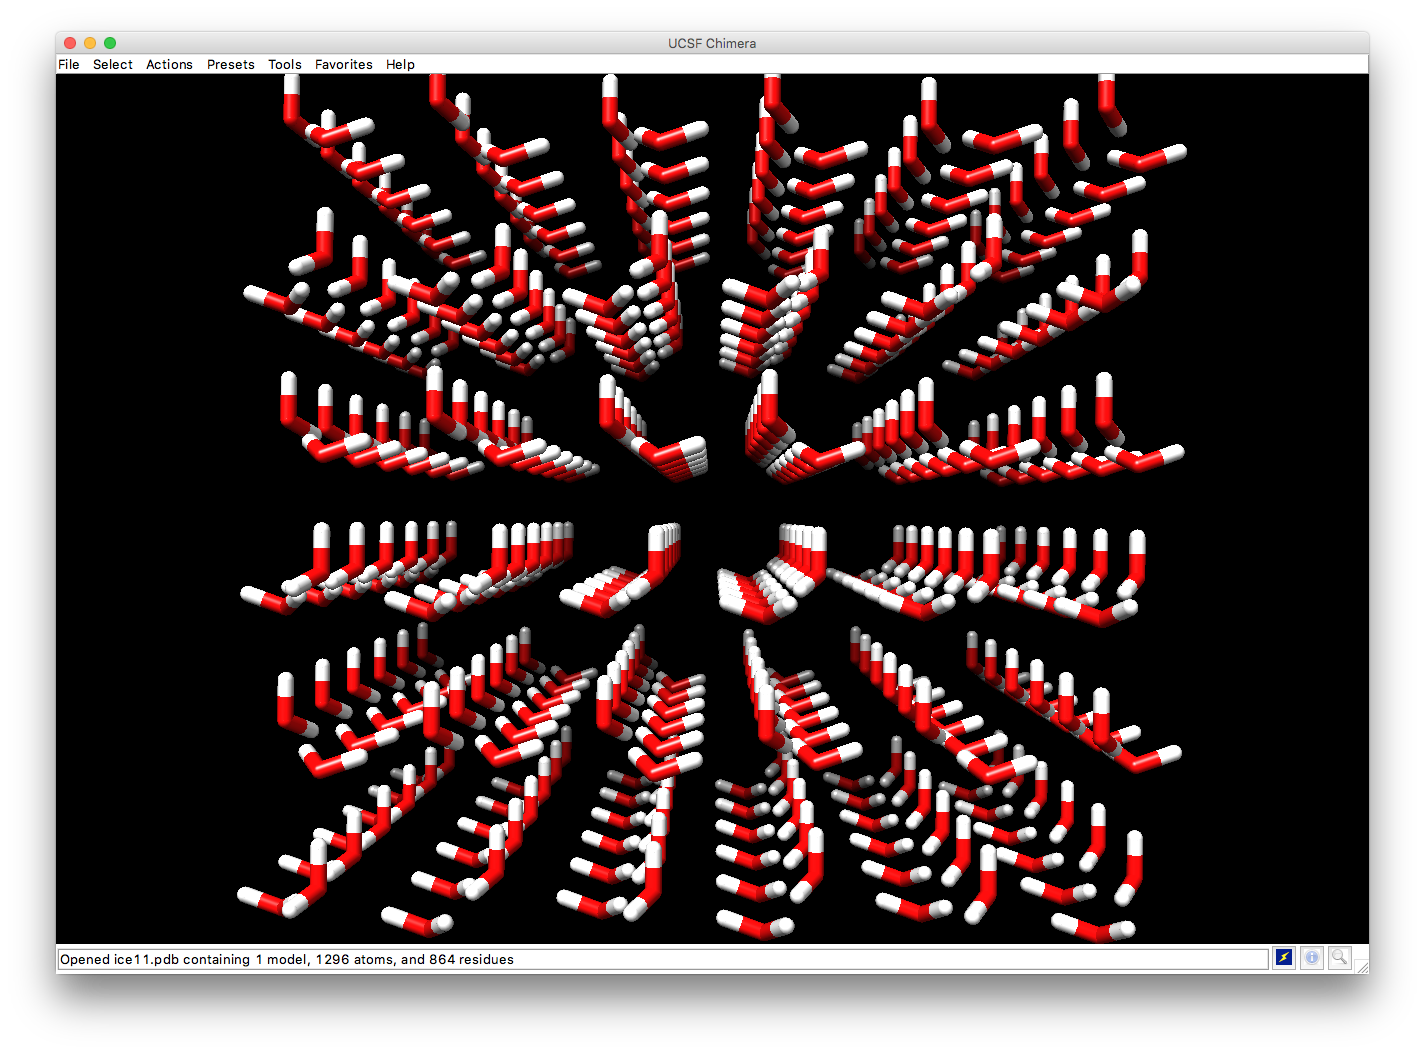
\includegraphics[width=0.75\textwidth]{iceXI.png}
	
	\caption{"Before" image of Ice XI}
	
	\label{fig:iceXI}
	
\end{figure}
\begin{figure}
	
	\centering
	
	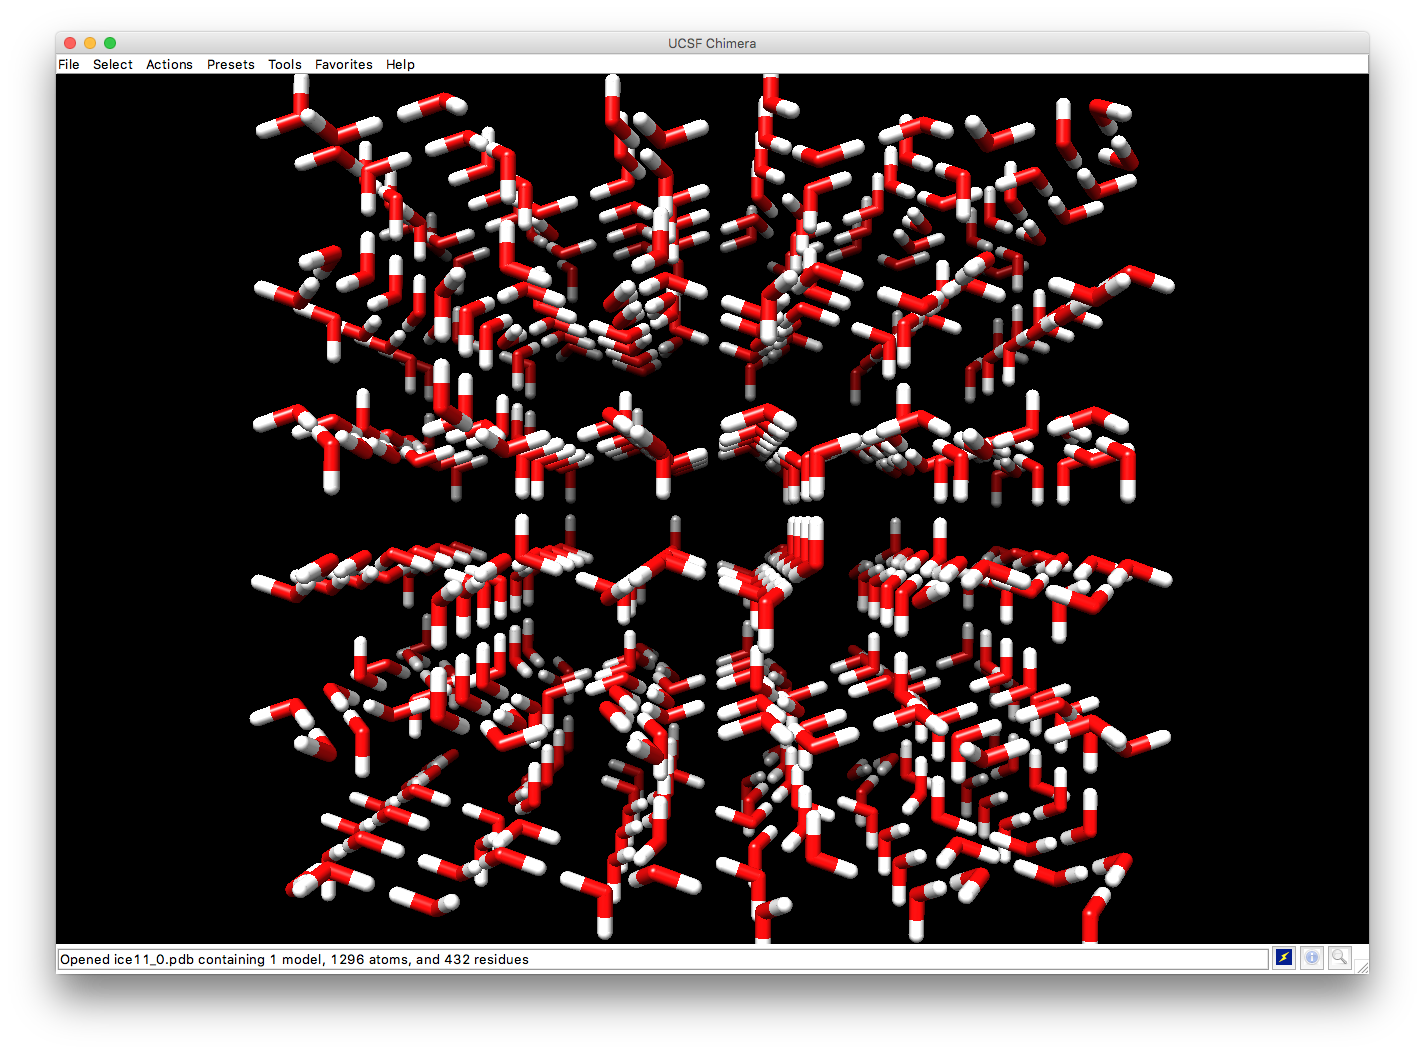
\includegraphics[width=0.75\textwidth]{iceIh.png}
	
	\caption{"After" image of generated ice Ih}
	
	\label{fig:iceIh}
	
\end{figure}
% FIX BELOW
As can be seen, the "after" image has experienced rotation and can no longer be classified as ice XI. 
However, as ice I$_{h}$ also has a standard shape, the generated crystal can not be considered ice I$_{h}$.
Instead, it can be considered a proton-disordered orthorhombic ice crystal similar to ice I$_{h}$. 

Unfortunately, the result is not without defect.
When following the subsequent layers in the crystal, patterns emerge. 
Inconsistently, some rows of waters remain consistent.
Some of these are a uniform rotation of both hydrogen atoms, while others are just one consistently placed hydrogen atom.
Multiple trials yield internally unique results, yet all contain these strange consistencies.
This may be due to some accidental pattern in the method's implementation.

% FINISH
%
%
%
%
\section{Comparison with Other Methods}
% USE BUTH PAPER
Currently in progress, this section will primarily compare the results of this method with \cite{MCIce}.
\subsection{benefits of own method over others}
\subsection{benefits of other methods over this}
%
%
%
%
% FINISH


\section{Comments on Limitations and Proposed Improvements}

During the hydrogen bond defect correction step, a weakness in the design is that any clustering or regions of high defect density will not be noticed.
This allows the existence of a highly-defective region within the larger structure that could potentially cause problems when the crystal is used in simulations. 
The prevalence and occurrence of these defects have not been studied, but seem a natural inevitability of statistics. 
% SHOW THE STATS
A potential solution with partial development will score regions based on the number of defects as a weighted function expanding out from a central molecule for N connections. 
For example, consider a given molecule defined as level 1. 
The neighboring four molecules are defined as level 2, and continued onward excepting already-defined molecules out to an N$^{th}$ level. 
The number of defects in each level can be counted and averaged.
Then a depressive factor along the lines of $\frac{1}{level}$ can be used to diminish the value of defects further away from the first-level molecule.
This would create a value for each molecule that shows the relative density of defects centered about that specific molecule and could even be plotted as a gradient change within the crystal.
The general approach to a scoring mechanism may take a form similar to equation \ref{eq:IceScoring}.
\begin{equation}
\label{eq:IceScoring}
Value = \sum_{l=1}^{N_{levels}} \Big[\frac{1}{l} * \frac{1} {N_{molecules}} *\sum_{m=1}^{N_{molecules}}[N_{defects, m}]\Big]
\end{equation}







\chapter{Crystal and Liquid 2D Water at Interfaces}
\label{ch:2DWater}


\section{Two-Dimensional Water}

EACH SUBSECTION: DEFINITION OF TERMS

Rose water is fairly new on the computational scene and so I may also include a review on the Mercedez-Benz water system as well as any other attempts to model water in two dimensions. For the rose potential system, I will review the Lennard-Jones potential  as well as any other equations/systems related to the rose potential.

\subsection{Lennard-Jones Potential}

The Lennard-Jones Potential well is a soft-sphere model of interaction between two spheres described with:

\begin{equation}
V_{LJ} = 4\epsilon[(\frac{\sigma}{r})^{12} - (\frac{\sigma}{r})^{6}]
\end{equation}
where $V$ is the potential, $r$ is the distance between the center of two particles , $\sigma$ is the specific distance between the two particles where the potential is zero, and -$\epsilon$ is the minimum potential of the plot.
\textbf{REFINE WORDING:}
The plot is defined in $[0,\infty)$.
As two particles approach from infinity, their interaction become negative - which is an attractive force - and will approach the global minimum of -$\epsilon$.
The $r$ of this interaction is slightly larger than the combined radii of the two particles - which means they aren't quite touching - and is the equilibrium distance between the two particles.
As $r$ decreases beyond the minimum and toward $\sigma$, the interaction strength increases and reaches zero as $r = \sigma$.
At $r < \sigma$, 

Potential digression:
In a "hard-sphere" model, a particle's radius is firm, which is to say that the interaction potential is infinite at $r$ less than $\sigma$. 
Basically a vertical line between two discrete values (usually $\epsilon$ and $\infty$)as the potential shifts from $r \geq \sigma$ to $r < \sigma$ (maybe include image?).
The Lennard-Jones potential is a "soft-sphere" model, which blurs the line and replaces the vertical line with a functional representation. 
This breaks with reality as the particles become "squishy" and the potential ramps up toward infinity as $r$ decreases. 
The benefit to the soft-sphere model is that modeling programs can more-easily account for overlaps in particles during time steps than with hard-sphere models. 
For example, a hard-sphere model of two particles interacting will likely not have a position where $r = \sigma$ and will potentially overlap. 
At this overlap, the potential is infinity and will introduce a nearly infinite force at that instant of time. 
Computer systems do not like having infinitely large repulsions suddenly introduced into a simulation. 


\subsection{Modeling Water in Two Dimensions}

Modeling in two dimensions sacrifice the "realism" of models in three dimensions, but reduce the computational load significantly.
This allows researchers (scientists, chemists, digital magicians?) to test more simple designs in two dimensions as well as a higher volume of simulations at the same time/computational cost. 


\subsubsection{Mercedes-Benz Model}

The "Mercedes-Benz" BN2D model of water first proposed by \cite{MBWater} as "waterlike particles" are a popular two-dimensional representation of water. 
ROUGH:
details of shape of MB water

The mathematical model used in the BN2D model is generated from the Percus-Yevick equation by substituting the approximation

\begin{equation}
c(X_{1}, X_{2}) = y(X_{1}, X_{2})f(X_{1}, X_{2})
\end{equation}

into the Percus-Yevick equation obtained from the Ornstein-Zernike relation 

\begin{equation}
h(X_{1}, X_{2}) = c(X_{1}, X_{2}) + \frac{\rho}{2\pi}\int c(X_{1}, X_{3}) h(X_{3}, X_{2})dX_{3}
\end{equation}

to produce the overall relation

\begin{equation}
y(X_{1}, X_{2}) = 1 + \frac{\rho}{2\pi}\int y(X_{1}, X_{3})f(X_{1}, X_{3}) \times \Big[ y(X_{3}, X_{2})f(X_{3}, X_{2}) + y(X_{3}, X_{2}) - 1 \Big] dX_{3}
\end{equation}


\subsubsection{Rose Potential Model}

The rose potential is another model first introduced by \cite{RoseOG}.
This model, while similar to the three-pronged BN2D, is notably different in that the rose potential model simplifies the model by use of a radial sinusoidal plot to make the three "prongs" of the particle. 

\subsubsection{Two-Dimensional Modeling}

Something other than OOPSE? (not seeing obvious answer other than "custom code modified/forked from existing 3D tools")

The Object Oriented Parallel Simulation Engine (OOPSE) was introduced by \cite{OOPSE} as a relatively light-weight molecular dynamics simulation package focused on "efficiently integrating equations of motion for atom types with orientational degrees of freedom" (from abstract).
While OOPSE was further developed and renamed OpenMD, a fork of OOPSE was developed specifically to model water in two dimensions.

\section{Objectives}

The objective of this work was to model two-dimensional water with a surface designed to discourage crystal growth at freezing temperatures. 
The design of the surface was the primary focus. 
Successfully designing a surface capable of discouraging water ice formation at freezing temperatures would provide valuable information in designing a three-dimensional model of the same type at a reduced computational cost. 

Idea: adjust freezing point depression to be freezing point modification.

\section{Tools and Terms}

Either a refresh from intro or a detailed explanation of OOPSE and the reduced terms.

% OOPSE
% 2D SYSTEMS
% 2D OOPSE
Detail differences in computation system that Dr. Fennell developed to allow 2D MD(?) on a 3D program.

\subsection{Reduced Terms: 2D analogues}

Detail differences in dimensionality and define the reduced dimensions. Still working on the understanding/equations.

\section{Designing System}

Include: 
ensemble, 
thermodynamic variables, 
box attributes (size, pressure, temp, etc), 
number of waters,
surface (size, spacing between beads of surface, charges, LJ values, etc)

\subsection{Defining the Surface}

Explain how to develop the surface in the program and how to build a custom surface 
% walk through surface builder here

\subsubsection{Manipulation of LJ Potential}

Manipulate $\sigma$ and $\epsilon$ values to effectively adjust the radius and interaction strength of surface beads.

\subsubsection{Manipulation of bead spacing}

Detail design of optimizing bead spacing for freezing encouragement or disruption.

\subsection{NEEDANOTHER}



\section{Results}

Success of freezing point elevation, pending results for freezing point depression




\chapter{Germanium Compounds and QM Concerns}
\label{ch:Germanium}

\section{Modeling Germanium Compounds}

While primarily used in optical applications including fiber optic cables and solar cell systems, germanium-based compounds are also used as polymerization catalysts.
Relative to many other elements on the periodic table, computational reports on germanium are not common.
Recent works have shown germanium's potential to polarize light.

% This will be an interesting section as there is extremely little in terms of Ge computational work. Perhaps a broader search will yield interesting results. For sake of thoroughness, I will also include work on computational energy optimization in general and work through complications brought by the size of Ge. I might also include a portion on the statistical spread of conformations at a given temperature (internal energy?) I may include a sentence or paragraph on Gaussian-based publications. 

\subsection{Computational Complexity of Germanium Compounds}

Publications on germanium computational efforts are not as common as many other main group elements. 
Of those extant publications, the majority of final published data involve a Density Functional Theory (DFT) with either the 6-31G(d), 6-31G(d,p), or 6-311G(2d) basis set.\cite{GeCompStudy1}
As with most other lighter elements calculated with Pople basis sets, the 6-31G(d,p) basis set is most commonly used for the final energy calculation.
% WHY THIS? 
% D AND P POLARIZATION INCLUDED IN CALCULATION - WHAT DOES THIS MEAN?

\section{The Initial Problem: Germanium Study}

During Fall 2017, Dr. Christopher Fennell was approached by Dr. Charles Weinert of OSU to continue a collaborative effort in sampling conformation energies of two germanium-based compounds of interest to Dr. Weinert's work. 
Seen as an opportunity to train a new graduate student in conformational calculations, this project was delegated to me.
The initial focus was to create the two compounds in a 3D modeling program, save a file of each, run a conformation optimization program on a supercomputer, and read the output to report the findings.
As detailed below, this work led to impossibilities, curiosities, and inconsistencies that resulted in a general solution and a discovery of a flaw in a popular computational program.

\subsection{Parameters of Work and Previous Collaborator's Results}

The two subject germanium-based compounds are very similar: a germanium backbone with terminal isopropyl groups and internal phenyl rings. 
One compound constituted a pentagermanium chain while the other a hexagermanium backbone. 
The molecular formula for both is $Pr^{i}_{3}Ge(GePh_{2})_{n}GePr^{i}_{3}$ where n equals 3 for the pentagermanium or 4 for the hexagermanium compounds, respectively.
An example image of both compounds in their fully-trans configurations are provided in figures \ref{fig:Ge5TransAll} and \ref{fig:Ge6TransAll}.

\begin{figure}
	
	\centering
	
	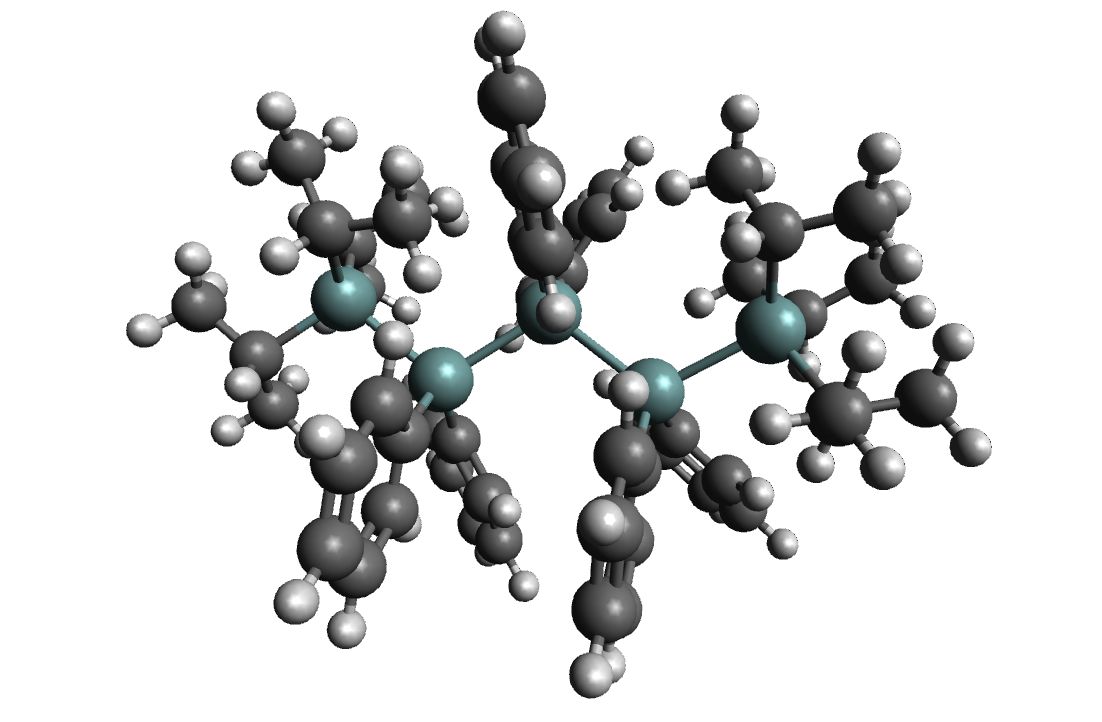
\includegraphics[width=0.75\textwidth]{5geTTT.png}
	
	\caption{Fully trans configuration of pentagermanium-based compound.}
	
	\label{fig:Ge5TransAll}
	
\end{figure}

\begin{figure}
	
	\centering
	
	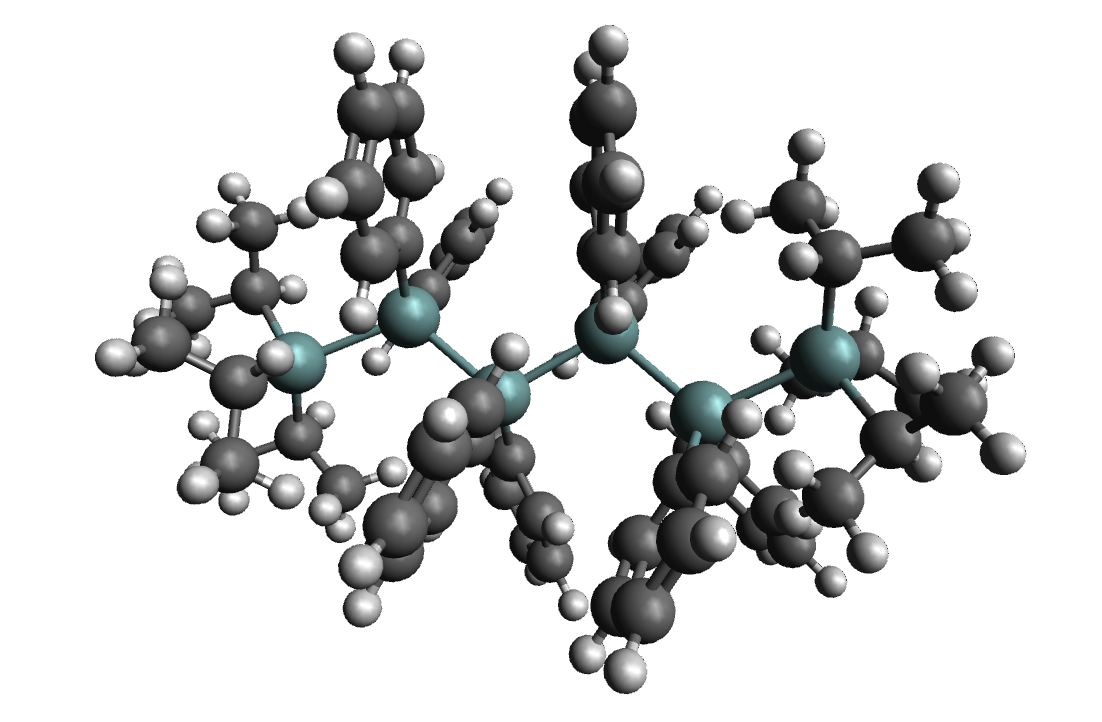
\includegraphics[width=0.75\textwidth]{6geTTT.png}
	
	\caption{Fully trans configuration of hexagermanium-based compound.}
	
	\label{fig:Ge6TransAll}
	
\end{figure}
\begin{table}[]
	
	\centering
	\begin{tabular}{llll}
		Conformation & Energy ($E_{h}$)    & $\Delta$ Energy ($E_{h}$) & $\Delta$ Energy ($\frac{kJ}{mol}$) \\ \cline{1-4} 
		Trans-coplanar        & -15014.8403143 & 0.0066255            & 17.39525025                        \\
		Cis-Trans-Cis         & -15014.7983311 & 0.0486087            & 127.6221418                        \\
		Trans-Cis-Trans       & -15014.8469398 & 0.0000000            & 0.0000000                                  \\
		Cis-Trans-Trans       & -15014.8246918 & 0.0222480            & 58.412124                         
	\end{tabular}
	\caption{Collaborator's Hexagermanium Energies by Conformation \\ (density functional theory, unknown basis set, energy in Hartrees and kJ/mol)}
	
	\label{tab:Ge6CollabEnergies}
	
\end{table}
Dr. Weinert had worked previously with a collaborator who provided conformation data supplied in table \ref{tab:Ge6CollabEnergies}.
While the basis set was not explicitly provided, it is likely that the most common 6-31G(d,p) basis set was used. 
Unfortunately, the collaborator is no longer active in research and was inaccessible for clarification.

The approach of labeling the conformation shape of each compound, given the many points of torsion, focuses on the backbone structure. 
As the raw data from the collaborator was not available, the general dihedral angles of cis and trans proved a vexing focus for initial efforts at conformer design.
Using Newman projections like in figure \ref{fig:Newman} as a visual guide, each Ge-Ge bond was defined as cis or trans based on the relative angle produced by the two  adjacent bonded Ge atoms to each subject Ge.
Specifically, the bonds are marked cis if the most acute angle is 90$^{\circ}$ or fewer, and likewise trans if greater than 90$^{\circ}$ up to the maximum 180$^{\circ}$.
Effectively the cis and trans angles coincide with gauche and anti in organic structure nomenclature.
Terminal germanium atoms are not considered as a part of the conformation state. 
This is partly due to the definition in labeling where the terminal germanium does not have an adjacent germanium for the measured relative angle, in addition to the assumed 
% CONFIRM GROUP THEORY - possibly S3?
C$_{3}$
% CONFIRM GROUP THEORY
symmetry of the terminal Ge with three isopropyl groups reducing the relative effects of terminal germanium rotation.
Effectively, only dihedrals formed by four consecutive Ge are given a cis or trans label.

\begin{figure}
	
	\centering
	
	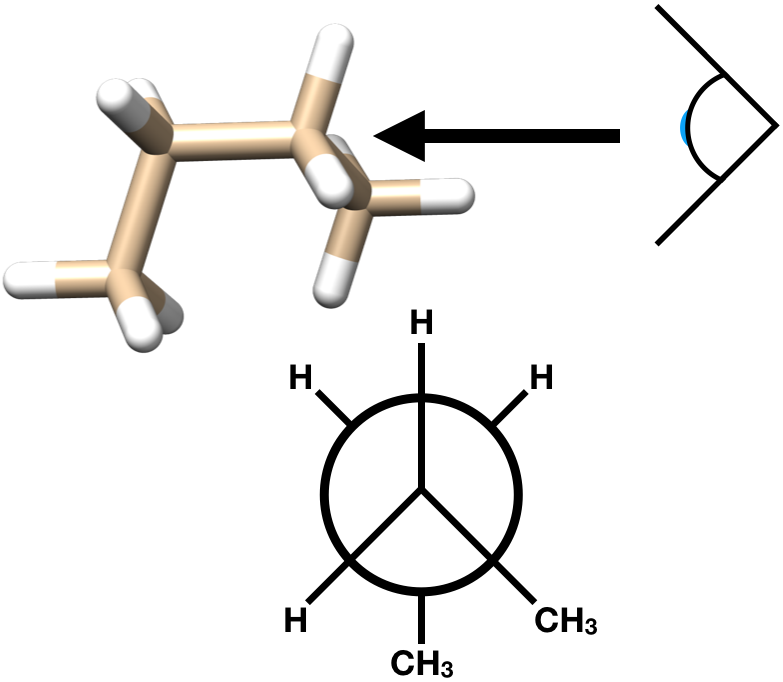
\includegraphics[width=0.75\textwidth]{NewmanCis.png}
	
	\caption{Sample Newman projection of cis-butane.}
	
	\label{fig:Newman}
	
\end{figure}

\subsection{Design and Approach to Solution}

The initial approach involved an attempt at basic replication of the collaborative results.
As detailed below, the design gradually grew in complexity as a learning process. 
Eventually, curiosities in results and a desire to automate an objective search algorithm developed into two unique investigations.

\subsubsection{Design 1: Occam's Smallest Razor}

With each non-terminal Ge-Ge dihedral initially labeled cis or trans for 0$^{\circ}$ or 180$^{\circ}$, about 3 unique pentagermanium and 6 unique hexagermanium structures were built visually on a 3D visualization program (Avogadro).
These were rotated without consideration for the phenyl rings populating the non-terminal Ge atoms.
Each molecule was subjected to an energy minimization in Gaussian 09 with the B3LYP hybrid function and STO-3G basis set as a single particle in a vacuum at otherwise default settings. 

Unsurprisingly, only the fully trans conformers successfully converged (a 22\% success rate) into a stable form. 
These troubles were likely caused by the poor design of the initial conformers. 
With initial results, the conformer design was altered into a more systematic approach with some consideration for the phenyl rings.

\subsubsection{Design 2: A Blunt Effort}

In the second iteration of the conformer design process, a greater number of backbone conformers were generated. 
Instead of the simple 180$^{\circ}$ opposition between the cis and trans conformers, more intentional initial angles seen in Newman projections were selected.
Specifically, the anti and both gauche angles were chosen for the natural local minima in a non-bulky molecule, with both gauche angles (60 and 300) labeled as cis and the anti angle (180) as trans. 
For initial conformer design, these backbone angles were limited to three positions: 60$^{\circ}$, 180$^{\circ}$, or 300$^{\circ}$.
For the hexagermanium compound, these structures were sequentially labeled trans-trans-trans, trans-trans-cis, trans-cis-trans, et cetera until all major unique conformers were produced.
For clarity, each conformer was identified by the dihedral angles (60-60-60, 60-60-180) in increasing order (Ge 1-2-3-4, Ge 2-3-4-5, Ge 3-4-5-6 dihedral).
The phenyl rings on the non-terminal Ge atoms were left untouched from an initial steepest-descent minimization available from Avogadro ran in the fully trans conformer.

To prevent potentially strong interactions between adjacent phenyl rings, an additional steepest-descent minimization from Avogadro was initially ran with the conformer-defining Ge-Ge dihedral angles locked in place. 
Additionally, a visual inspection of the phenyl rings and manual adjustments were utilized on Avogadro to reduce the chance of a relatively high energy local minima conformer. 
The phenyl rings usually were settled in a form of pi stacking or some kind of perpendicular ring interaction, based on relative energy stability according to the immediate simple minimization available. 

To further avoid backbone rotation restrictions, variations of the bulky molecules were also produced. 
These included versions where the phenyl rings were replaced by methyl groups and also where the isopropyl ends were additionally replaced by methyl groups. 
There intention in these designs were to observe the shift in relative energy between the sets of conformers to determine how significant of a role the phenyl rings and isopropyl groups played.
These variations, along with the original form structures, were subject to the same calculations as in the first design: Gaussian 09, B3LYP hybrid functional, STO-3G basis set, no angle restrictions, single particle in a vacuum, otherwise default parameters.
The results of these calculations are tabulated in tables \ref{tab:Ge5Ver2Data} and \ref{tab:Ge6Ver2Data}.

\begin{table}[]
	\centering
	\begin{tabular}{llllll}
		\begin{tabular}[c]{@{}l@{}}Internal\\ Species\end{tabular} & \begin{tabular}[c]{@{}l@{}}Terminal\\ Species\end{tabular} & Conformer & \begin{tabular}[c]{@{}l@{}}Final Energy\\ (Hartrees)\end{tabular} & \begin{tabular}[c]{@{}l@{}}∂ Energy\\ (Hartrees)\end{tabular} & \begin{tabular}[c]{@{}l@{}}∂ Energy\\ (kJ/mol)\end{tabular} \\ \hline
		methyl & methyl & 60-60 & -10738.91336 & 0.0000454 & 0.119 \\
		methyl & methyl & 60-180 & -10738.9134 & 0 & 0 \\
		methyl & methyl & 60-300 & -10738.91286 & 0.0005358 & 1.407 \\
		methyl & methyl & 180-60 & -10738.91325 & 0.0001533 & 0.402 \\
		methyl & methyl & 180-180 & -10738.91335 & 0.0000475 & 0.125 \\
		methyl & methyl & 180-300 & -10738.91336 & 0.0000451 & 0.118 \\
		methyl & methyl & 300-60 & -10738.91336 & 0.0000455 & 0.119 \\
		methyl & methyl & 300-180 & -10738.91287 & 0.0005357 & 1.406 \\
		methyl & methyl & 300-300 & -10738.9107 & 0.002703 & 7.097 \\ \hline
		phenyl & methyl & 60-60 & -11875.15183 & 0.0001451 & 0.381 \\
		phenyl & methyl & 60-180 & -11875.15144 & 0.0005304 & 1.393 \\
		phenyl & methyl & 60-300 & -11875.15197 & 0 & 0 \\
		phenyl & methyl & 180-60 & -11875.14282 & 0.0091505 & 24.025 \\
		phenyl & methyl & 180-180 & -11875.15004 & 0.0019354 & 5.081 \\
		phenyl & methyl & 180-300 & -11875.15064 & 0.0013353 & 3.506 \\
		phenyl & methyl & 300-60 & -11875.06665 & 0.0853257 & 224.023 \\
		phenyl & methyl & 300-180 & DNC & DNC & DNC \\
		phenyl & methyl & 300-300 & -11875.1497 & 0.0022723 & 5.966 \\ \hline
		phenyl & isopropyl & 60-60 & DNC & DNC & DNC \\
		phenyl & isopropyl & 60-180 & -12341.23176 & 0.0053028 & 13.923 \\
		phenyl & isopropyl & 60-300 & DNC & DNC & DNC \\
		phenyl & isopropyl & 180-60 & DNC & DNC & DNC \\
		phenyl & isopropyl & 180-180 & -12341.23513 & 0.001935 & 5.08 \\
		phenyl & isopropyl & 180-300 & DNC & DNC & DNC \\
		phenyl & isopropyl & 300-60 & DNC & DNC & DNC \\
		phenyl & isopropyl & 300-180 & -12341.23706 & 0 & 0 \\
		phenyl & isopropyl & 300-300 & DNC & DNC & DNC
	\end{tabular}
	\caption{Data of B3LYP/STO-3G minimization of variations of pentagermane compound at various conformers. DNC denotes a failure to converge with the self-consistent field method.}
	\label{tab:Ge5Ver2Data}
\end{table}

\begin{table}[]
	\centering
	\begin{tabular}{llllll}
		\begin{tabular}[c]{@{}l@{}}Internal\\ Species\end{tabular} & \begin{tabular}[c]{@{}l@{}}Terminal\\ Species\end{tabular} & Conformer & \begin{tabular}[c]{@{}l@{}}Final Energy\\ (Hartrees)\end{tabular} & \begin{tabular}[c]{@{}l@{}}∂ Energy\\ (Hartrees)\end{tabular} & \begin{tabular}[c]{@{}l@{}}∂ Energy\\ (kJ/mol)\end{tabular} \\ \hline
		methyl & methyl & 60-60-60 & -12870.91834 & 0.0009503 & 2.495 \\
		methyl & methyl & 60-180-60 & -12870.91929 & 0.0000004 & 0.001 \\
		methyl & methyl & 60-180-180 & -12870.91813 & 0.0011628 & 3.053 \\
		methyl & methyl & 60-180-300 & -12870.91869 & 0.0005972 & 1.568 \\
		methyl & methyl & 60-300-300 & DNC & DNC & DNC \\
		methyl & methyl & 180-60-60 & -12870.91897 & 0.0003189 & 0.837 \\
		methyl & methyl & 180-180-60 & -12870.91833 & 0.0009585 & 2.517 \\
		methyl & methyl & 180-180-180 & -12870.91929 & 0.0000004 & 0.001 \\
		methyl & methyl & 180-180-300 & -12870.91929 & 0.0000003 & 0.001 \\
		methyl & methyl & 180-300-60 & -12870.91897 & 0.0003192 & 0.838 \\
		methyl & methyl & 300-60-180 & DNC & DNC & DNC \\
		methyl & methyl & 300-180-60 & -12870.91929 & 0 & 0 \\
		methyl & methyl & 300-180-180 & DNC & DNC & DNC \\
		methyl & methyl & 300-180-300 & -12870.91814 & 0.0011527 & 3.026 \\ \hline
		phenyl & methyl & 60-60-60 & DNC & DNC & DNC \\
		phenyl & methyl & 60-60-180 & -14385.89674 & 0.0052183 & 13.701 \\
		phenyl & methyl & 60-60-300 & -14385.89487 & 0.0070829 & 18.596 \\
		phenyl & methyl & 60-180-60 & DNC & DNC & DNC \\
		phenyl & methyl & 180-60-60 & DNC & DNC & DNC \\
		phenyl & methyl & 180-60-180 & -14385.90195 & 0 & 0 \\
		phenyl & methyl & 180-60-300 & -14385.89855 & 0.0033998 & 8.926 \\
		phenyl & methyl & 180-180-180 & -14385.83838 & 0.0635763 & 166.92 \\
		phenyl & methyl & 180-300-180 & -14385.79233 & 0.1096251 & 287.821 \\
		phenyl & methyl & 300-60-60 & DNC & DNC & DNC \\
		phenyl & methyl & 300-60-180 & -14385.89836 & 0.003597 & 9.444 \\
		phenyl & methyl & 300-60-300 & -14385.89836 & 0.0035979 & 9.446 \\
		phenyl & methyl & 300-180-60 & DNC & DNC & DNC \\
		phenyl & methyl & 300-300-300 & DNC & DNC & DNC \\ \hline
		phenyl & isopropyl & 60-180-180 & -14851.9865 & 0 & 0 \\
		phenyl & isopropyl & 60-300-60 & DNC & DNC & DNC \\
		phenyl & isopropyl & 60-300-180 & DNC & DNC & DNC \\
		phenyl & isopropyl & 180-300-60 & DNC & DNC & DNC \\
		phenyl & isopropyl & 180-300-180 & DNC & DNC & DNC \\
		phenyl & isopropyl & 180-300-300 & DNC & DNC & DNC \\
		phenyl & isopropyl & 300-300-60 & DNC & DNC & DNC \\
		phenyl & isopropyl & 300-300-180 & DNC & DNC & DNC \\
		phenyl & isopropyl & 300-300-300 & DNC & DNC & DNC
	\end{tabular}
	\caption{Data of B3LYP/STO-3G minimization of variations of hexagermane compound at various conformers. DNC denotes a failure to converge with the self-consistent field method.}
	\label{tab:Ge6Ver2Data}
\end{table}


Immediately obvious in the table are the considerable number of nonconverged results. 
An unexpected bulkiness trend followed that a fully methylated variation of the structure was most likely to converge to a stable state, while the fully internal phenyl structures with methyl ends slightly reduced convergence and the original fully internal phenyl structures with isopropyl ends drastically reduced convergence.
The common-sense expectation that the addition of the phenyl ends would reduce stability was not parroted in these results. 
A deeper exploration into the change of stability is a promising avenue for future investigation, but was not further explored in this work.
As can be seen in table \ref{tab:Ge6Ver2Data}, the lowest energy conformer for each structure varied greatly, but never included the fully trans conformer and only once the collaborator-reported trans-cis-trans conformer as the most stable.
Still, given the considerable amount of nonconverged conformers, a new design was necessary to further improve the scope of the lowest energy conformation search.

\subsubsection{Design 3: Death by 1.59 Million Cuts}

In the final version of the conformer generation effort, additional creation efforts were focused on the individual phenyl rings. 
The unfavorable interactions between the phenyl rings were considerable hurdle in the previous designs and a potential explanation for the large number of nonconverged structures, including the possibility that the terminal isopropyl hexagermanium structures contained particularly unfavorable interactions among the phenyl rings.
This third design sought to remove the uncertainty in phenyl ring bulkiness by applying the same approach as the backbone generation: create unique conformers of every backbone torsion and phenyl ring, limiting each torsion to one of three rotational positions following the Newman projection style. 
Unfortunately, this task proved prohibitively large.

As an explanation for the insurmountability of the problem, consider the hexagermanium structure. 
The germanium dihedrals represent three rotatable bonds each with three initial positions. 
To include the phenyl rings would require the inclusion of eight new rotatable bonds each with three initial positions.
Additionally, considering each terminal germanium's rotation while ignoring each isopropyl's rotatable bonds adds two initial positions each with three initial positions. 
Together, this creates a structure with 13 rotatable bonds each with three initial positions. The number of conformers follows as $3^{13} = 1,594,323$ initial conformers. 
Now we must consider the computational aspect of this many conformers.
At 10 conformers rotated and generated per second and 16 KB per conformer, the initial conformers would require 44.3 hours and generate 25.49 GB of data just in the initial structures.
At an average of 72 minutes per computation and 73.7 MB produced at B3LYP hybrid functional and STO-3G basis set and access to all 255 regular nodes of Oklahoma State University's Cowboy cluster running in parallel, the complete computation would generate 117.5 TB of data and require 312 days of continuous computation to determine a possible lowest energy conformer of this one molecule at a relatively low level basis set and theory.
A request to utilize 100\% of university supercomputer resources for nearly a year for the sake of determining the lowest energy conformer of one molecule would likely be rejected, so this task would likely require a time scale of years or even decades to produce with shared access to university resources. 
While conventionally considered a small molecule, the scale of conformers and computational requirements pushes this problem into the realm of Levinthal's paradox.

While this third design would have likely revealed the lowest energy conformer, or at least one considerably close the the exactly lowest energy conformer, the effort ultimate fails under its own weight.
Even with efforts to truncate duplicate forms, the problem of scale remains.
A reduction by 50\% still requires a computation effort in the timescale of years or decades for the calculation of a single molecule.
For an effective computational outlook, this system needs to be reduced by several orders of magnitude.

\subsection{Scale Reduction Efforts}

For a system with conformers on the millions scale and computations on the hour scale, a magnitude reduction in either aspect would improve the practicality of this design approach.
For example, by simplifying the computational method from 72 minutes on average to 5 minutes on average, the overall computational requirement would be reduced by 92\%, a full order of magnitude. 
Unfortunately, reducing the complexity of the method sacrifices the reliability of data.
A potential solution here would be to create rounds of calculations at different complexities, where each sequential round restricts the pool of potential conformers.
Ideally, the balance of the increasing computational complexity and the decreasing pool size would maintain a consistent computational requirement.
For example, a new round using a higher functional theory and basis set at 5x computational requirement would ideally be paired with a reduction in conformer pool size by a factor of 5.
This would produce a series of calculation sets with additive computational requirement instead of a magnitudinal expansion.

The natural next question lies within the reliability of basis sets and functional theories. 
It naturally follows that a less-accurate method should not be relied on while better methods exist. 
However, considering the scale of the conformer pool, it follows that a less accurate method would still produce energy values with a roughly similar internal consistency. 
For example, a 180-0-180 form of the hexagermanium compound with parallel phenyl rings as modeled in figure \ref{fig:6geTCT} will have intense syn interactions between some phenyl rings and will likely not yield a desirable energy value at any level of calculation while a fully trans form with perfect pi stacking phenyl rings will likely have a lower energy value at all levels of calculation.
It follows that, at lower levels of accuracy, the extremely high energy conformers can be pruned from the pool early and drastically reduce overall computational requirements.
A generic effort at producing a method in this style is detailed in chapter \ref{ch:ConformationLandscape}, while the remainder of this chapter details additional efforts of calculating these germanium compounds.

\begin{figure}
	
	\centering
	
	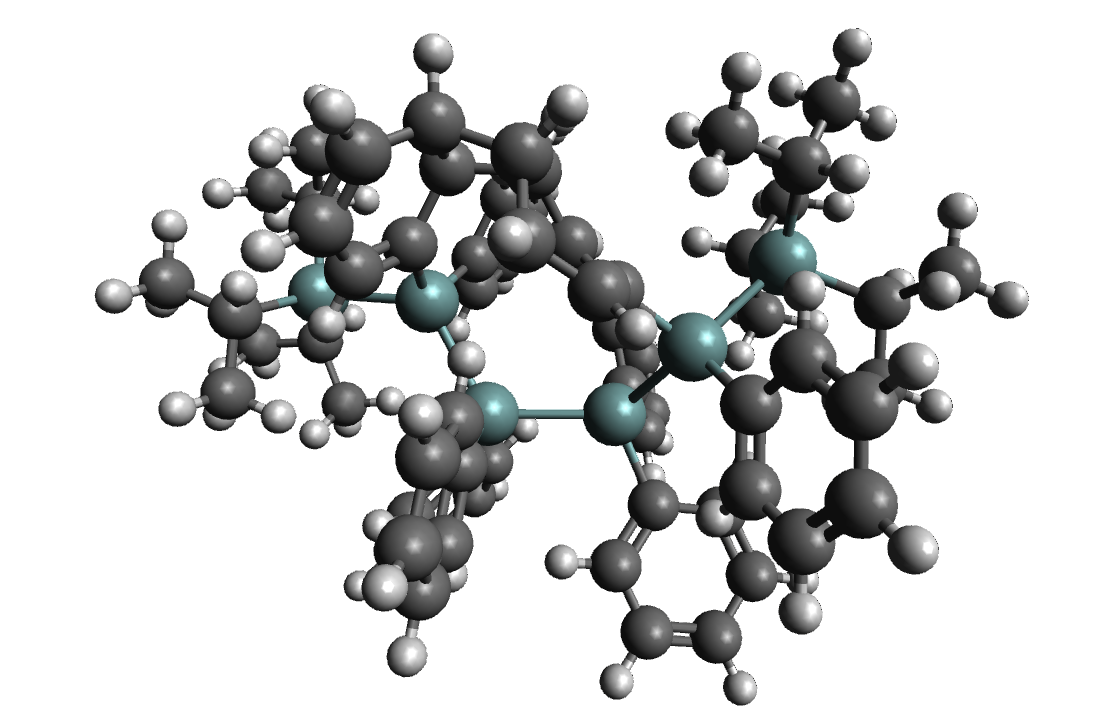
\includegraphics[width=0.75\textwidth]{6geTCT.png}
	
	\caption{Visualization of a trans-cis-trans hexagermane structure.}
	
	\label{fig:6geTCT}
	
\end{figure}

\subsection{Efforts at Simplification}

One potential avenue of simplifying the process is computing the energy minimizations of lower-period atoms (e.g. a carbon backbone instead of germanium) and then applying a correction factor for a net reduction in computation time.
As a period 4 element, germanium exhibits computational qualities similar to but more complicated than both carbon and silicon.
Using tested samples, an energy minimization of a carbon-backbone molecule instead of the germanium represented a 92\% reduction in computation speed.
Assuming a nominal correction factor exists and can be applied, this represents an order of magnitude reduction in computation time with one simplification. 
Potentially, this would allow investigators to much more quickly eliminate high energy conformers and more rapidly reduce the scope of the search.

The approach to acquiring sufficient data for a possible correction factor involved running an extremely simplified form of the germanium compounds, specifically a butagermanium backbone with hydrogens occupying all terminal and internal bonds.
This reduced the complication and complexity of bulkiness and allowed for quick full torsion rotations about the single Ge-Ge-Ge-Ge dihedral.
By operating at intervals of 5$^{\circ}$, a full torsion drive provides a glimpse at relative energies of the molecule at 72 discrete states. 

The extended round of torsion drive calculations included an alteration in representation of the data.
As the focus had shifted from relative energies and intensities across multiple theories and basis sets to a focus on graph smoothness and internal relative energies, the energy axis of plots were reduced to a unitless scale ranging 0 to 1, where 0 represents the minimum energy and 1 represents the maximum energy in a given set of torsion drive data.
This allowed for graphical representations of each torsion drive to emphasize the internal variation of torsions relative to the minimum and maximum values.
This was accomplished by taking any set of data with absolute scale energy unit, identifying the minimum and maximum values, and scaling each data point according to equation \ref{eq:TorsionReducedScale}. 
The script to collect and scale data points is detailed in \ref{ch:App:Germane}.

\begin{equation}
% NEEDS SOME WORK
E_{i, red} = \frac{E_{i,abs} - E_{min,abs}}{E_{max,abs}-E_{min,abs}}
\label{eq:TorsionReducedScale}
% NEEDS SOME WORK
\end{equation}

An example plot of this torsion drive is shown in figure \ref{fig:EXTorsion} Once multiple torsion drives had completed in multiple group four elements (butyl C, Si, and Ge were all built and tested), the energies could be compared and analyzed for any relative or absolute scaling at the additive or multiplicative reference. 
%MORE

\begin{figure}
	
	\centering
	
	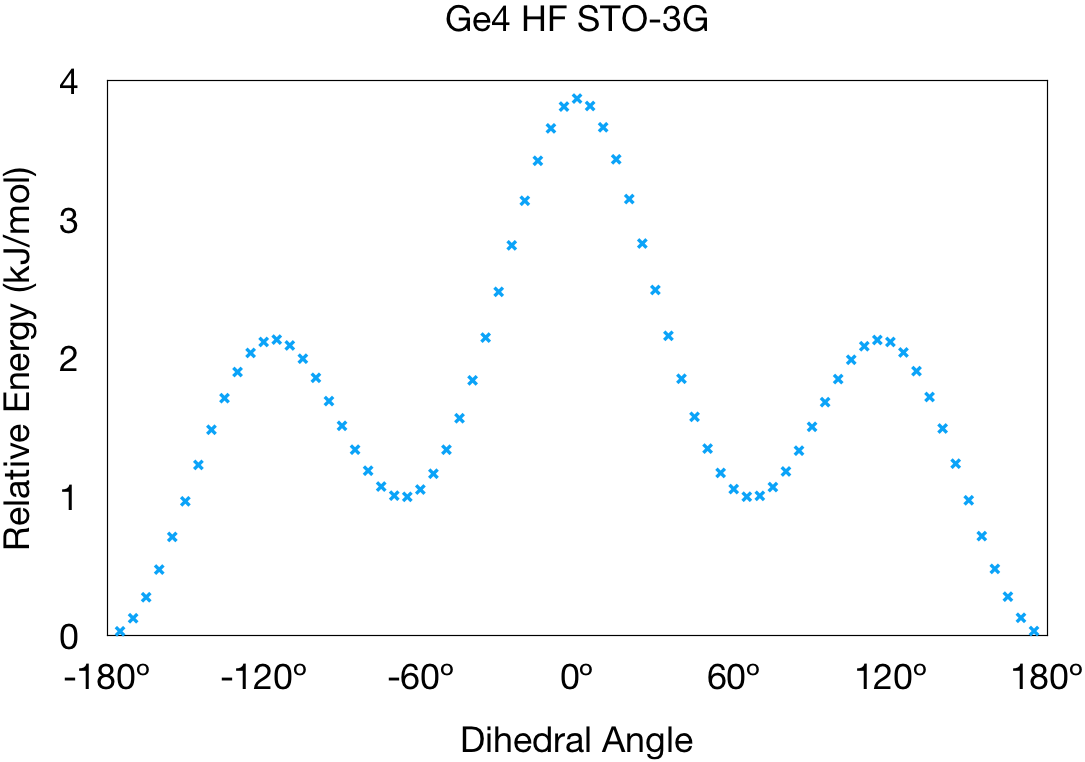
\includegraphics[width=0.75\textwidth]{Ge4HFSTO3G.png}
	
	\caption{Sample torsion plot at reduced energy scale.}
	
	\label{fig:EXTorsion}
	
\end{figure}

For a full comparative set, 3456 points of analyzed data were generated for each reference molecule's free energy in comparison with the others. 
Unsurprisingly, no simple correction factor arose by method of a simple additive or multiplicative term applied toward all torsion points. 
To expand on the comparative set, a set of butyl- group IV conformers were generated with every possible permutation of C, Si, and Ge, each then rotated about the torsion in 5$^{\circ}$ increments to produce a total 5832 conformers.
These were then subject to the same data comparison method as before, again to no noticeable trend.
A future avenue of research could be to further explore this with depressive or polynomial terms to discover whether a simple corrective function might exist with specific molecules.

While this approach likewise did not find any simple correction factor, a graphical representation of multiple functionals across the butyl C, Si, and Ge show an interesting trend, as visualized by a graph provided by Dr. Christopher Fennell and shown in figure \ref{fig:FennellTorsion}.
\begin{figure}
	
	\centering
	
	\makebox[\textwidth][c]{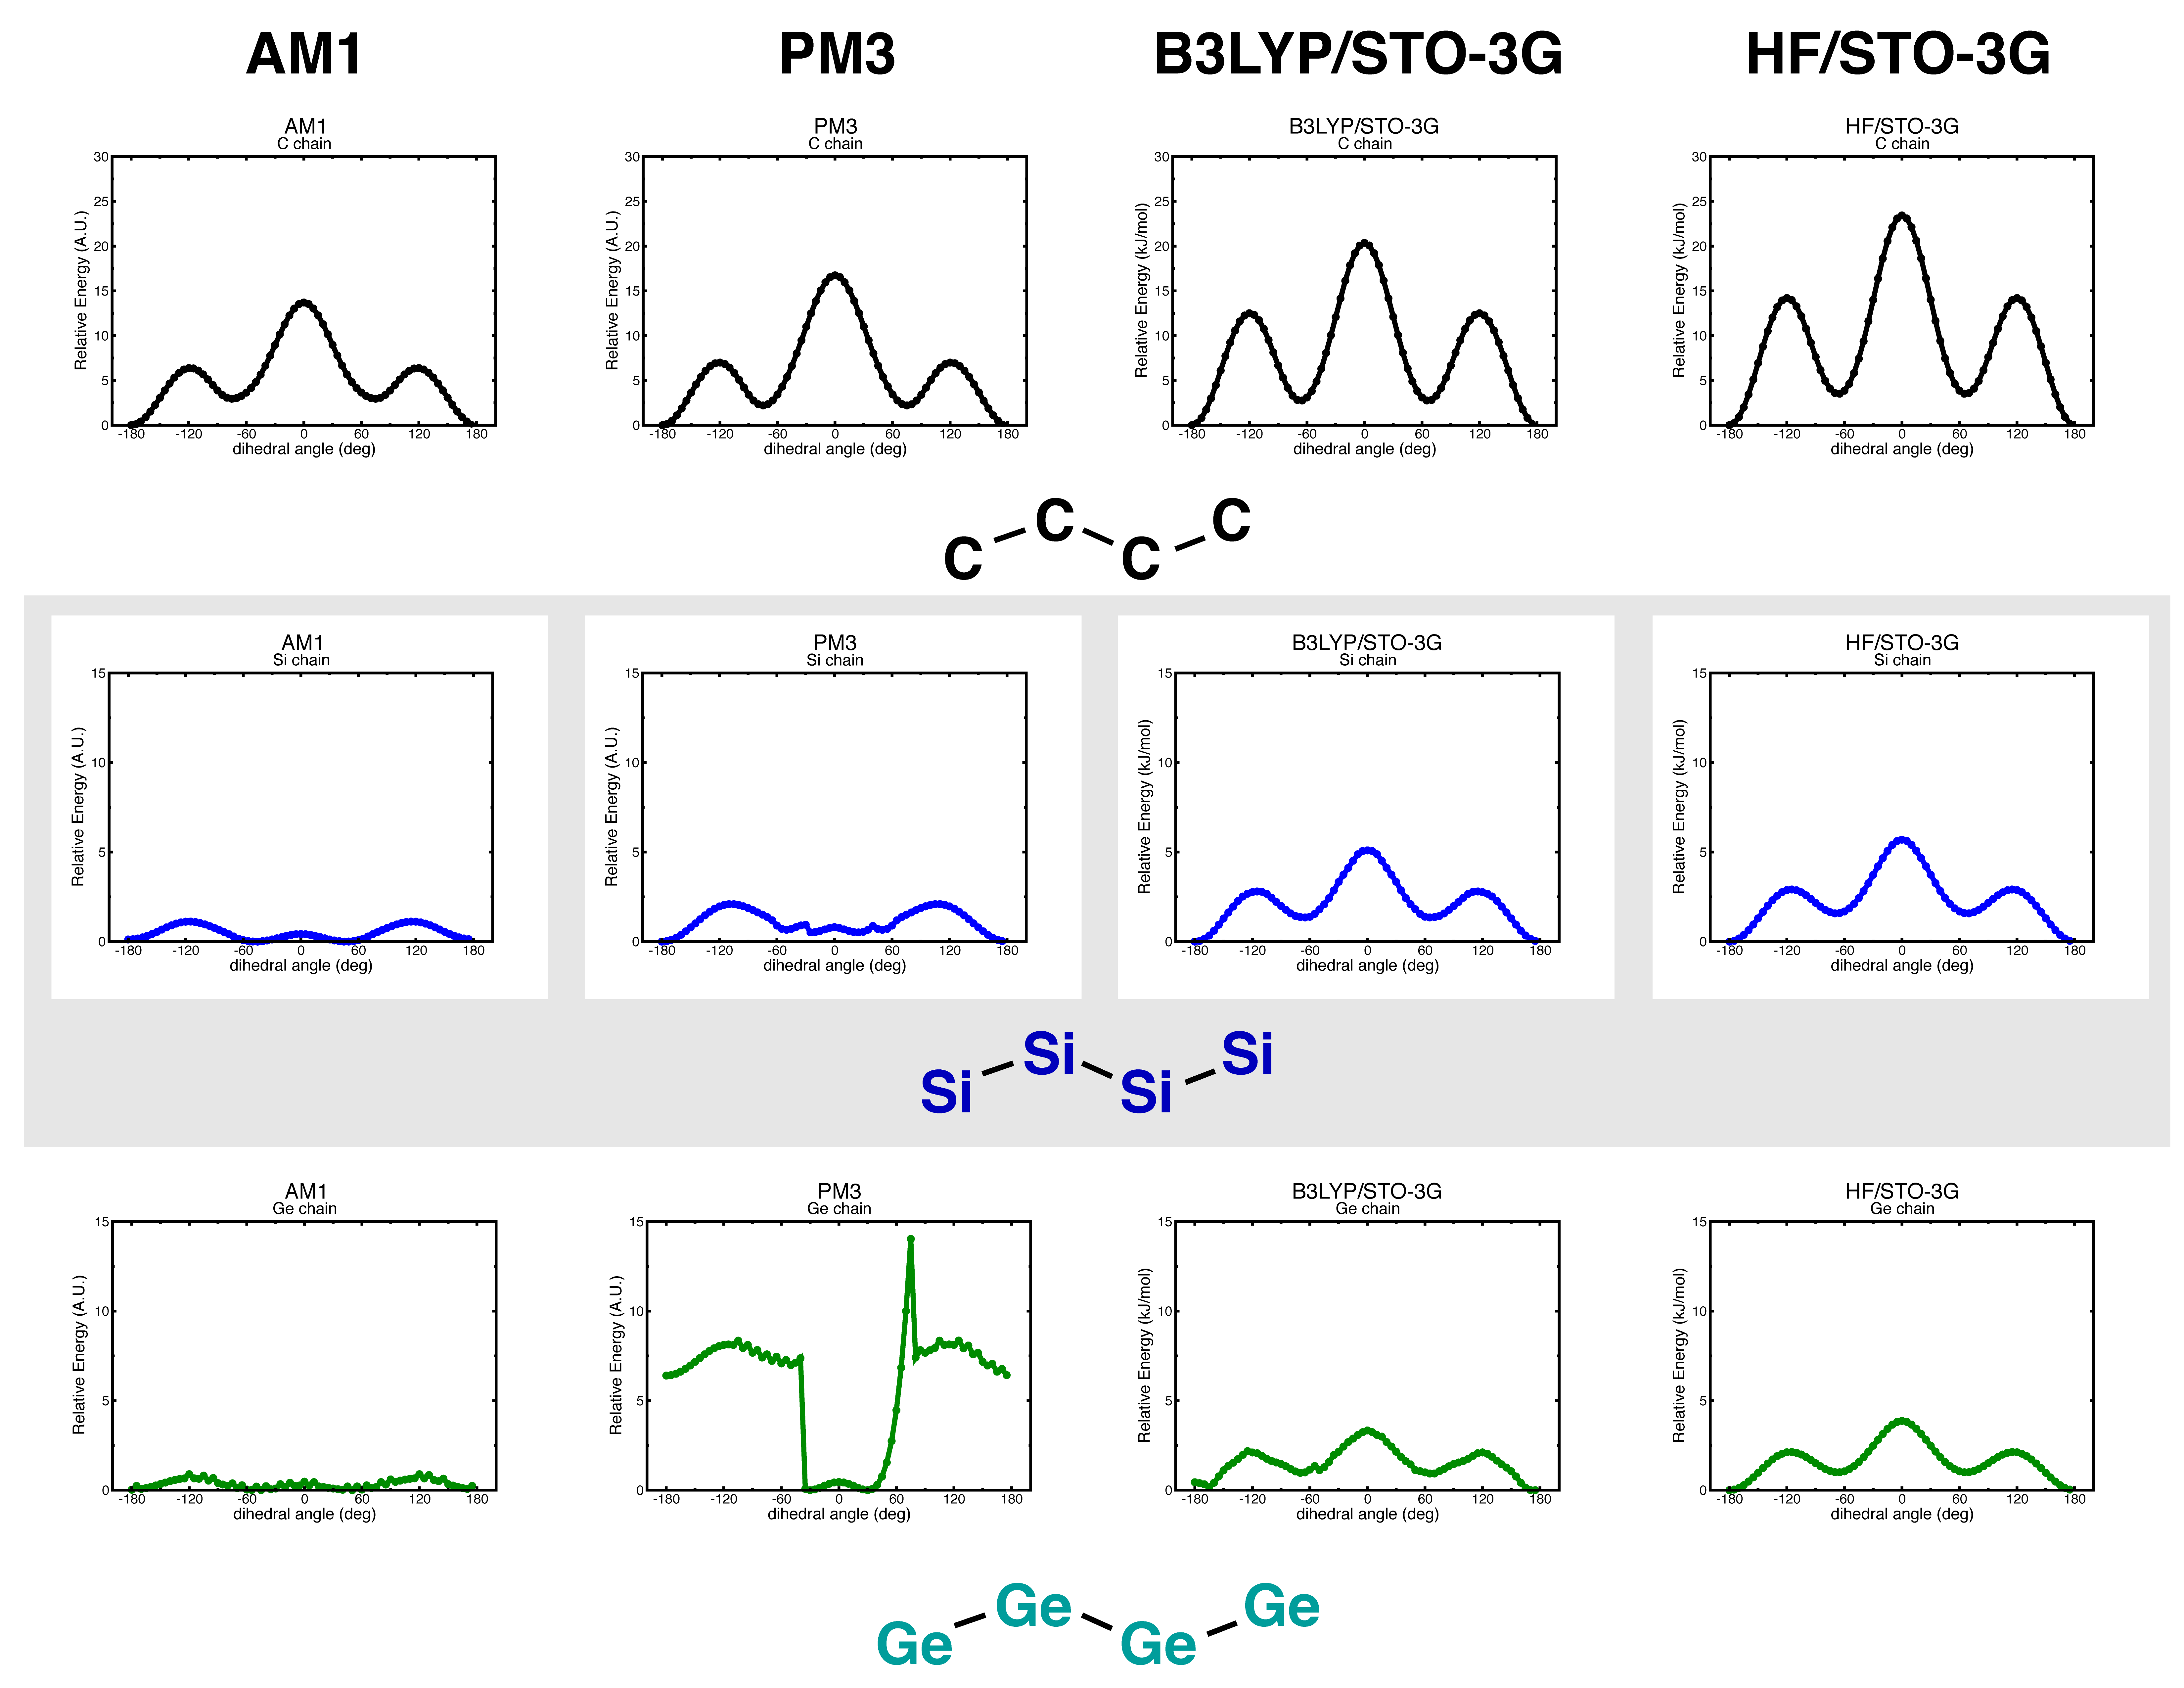
\includegraphics[width=1.3\textwidth]{FennellTorsion.png}}
	
	\caption{Visualization of a multiple pure group IV torsions at various theories and basis sets}
	
	\label{fig:FennellTorsion}
	
\end{figure}
A common theme of these graphs is that the relative energies follow the expected energetic barrier of a Newman projection, with local maxima at the 120$^{\circ}$ and 240$^{\circ}$ (or -120$^{\circ}$) angles and local minima at the 60$^{\circ}$ and 300$^{\circ}$ (or -60$^{\circ}$).
The global maximum and minimum were consistently at 0$^{\circ}$ and 180$^{\circ}$ angles, respectively.
As expected by different types of calculations, the torsion graphs hold different internal relative energies. 
For carbon, all four functionals produced a clean curve. 
The AM1 and PM3 functionals produced unexpected results for both Si and Ge graphs. 
In each, the expected highest energy 0$^{\circ}$ torsion angle was instead the most favorable of the three eclipsed angles.
Additionally, the Si PM3 and the Ge AM1 and PM3 functionals showed strong spikes along the expectedly smooth curve, with the Ge PM3 being noticeably broken.

While the Si graphs smoothed out for the B3LYP and HF functionals at STO-3G basis set, the Ge B3LYP showed significant spikes and only the HF STO-3G exhibited a smooth curve.
Effectively, this discovery of spikes along torsion drives led to the realization that the validity of a basis set could possibly be determined by the smoothness of a torsion drive.
For example, any calculation of a germanium-containing molecule will likely not produce reliable results with a B3LYP hybrid functional and STO-3G basis set, while the Hartree Fock STO-3G calculation would at least be tentatively reliable for comparative energy levels at various conformations.


\section{Discovery of a Consistent Inconsistency}

The next natural step was to calculate and plot additional functional theories and basis sets with the butagermanium chain. 
While effectively a lightly guided meandering through the available calculation types, the first effort was to observe relative differences across multiple basis sets of the Hartree Fock theory and to examine the relative computational requirements of each.
This plan was quickly redirected, however, when a curiosity within the data was revealed.

While running additional torsion drives of butagermane at differing basis sets and functional theories, an inverted energy was discovered. 
As can be seen in figure \ref{fig:geTorsFirst}, the B3LYP theory with 6-31G(d) basis set appears flipped upon a cursory glance. 
After a more careful observation, the minima and maxima are at the "wrong" angles and cannot be a simple flip of the minima and maxima.
Instead, the data is simply junk.

\begin{figure}
	
	\centering
	
	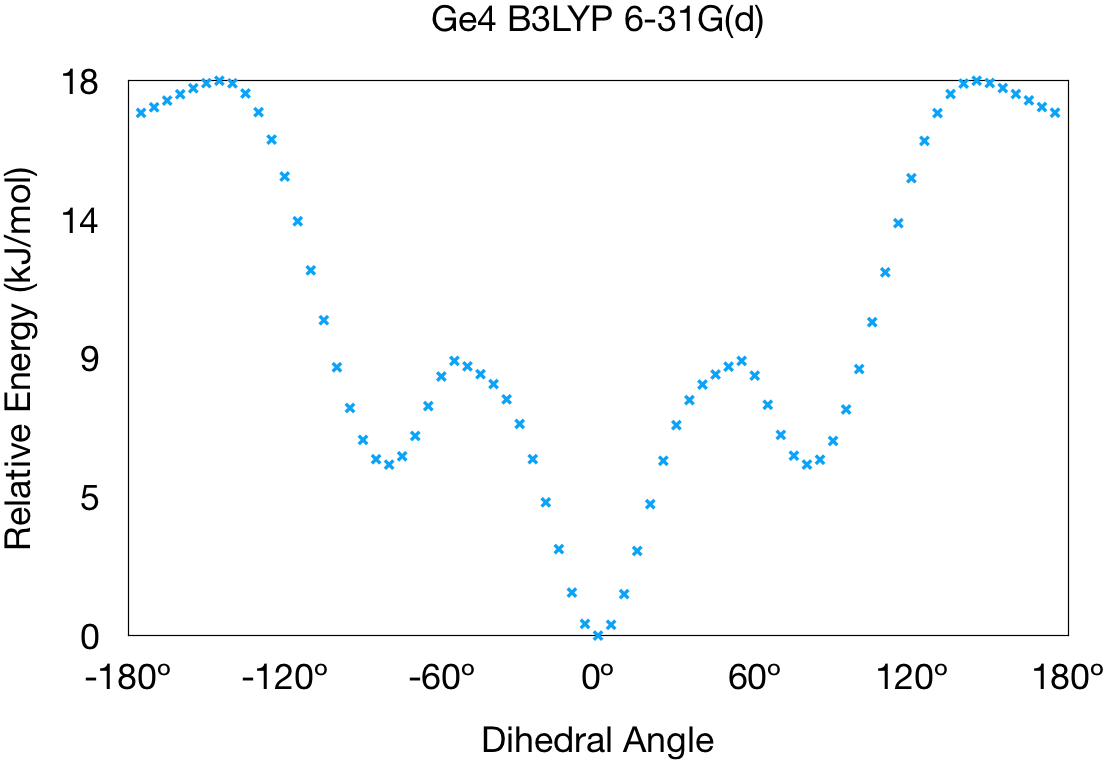
\includegraphics[width=0.75\textwidth]{geTorsFirst.png}
	
	\caption{A curious seemingly-inverted torsion plot of butagermane.}
	
	\label{fig:geTorsFirst}
	
\end{figure}

Naturally, the focus shifted toward discovering the source of the bad data.
A repeat of the trial yielded the same data.
A repeat of the system with a freshly created butagermane yielded the same data.
A trial with data from a butagermane trial with the 6-31G(d,p) basis set yielded the same data.
Each attempt at a 6-31G(d) basis set with the B3LYP theory yielded junk data, while other basis sets within the theory produced expected data. 
Next, the butagermane torsions were run with an identical basis set group with the Hartree-Fock theory, the results of which are shown in table \ref{fig:geTorsOne}.

Surprisingly, the 6-31G(d) result was also strangely inverted.
This process was repeated for several more theories, with the 6-31G(d) basis set results plotted in figure \ref{fig:geTorsAll}.
Curious to see if the germanium atom's basis set data or if the entire basis set method was the source, a similar run with butasilane was made and graphed in figure \ref{fig:siTorsOne}, to expected results.
A quick run confirmed the problem to also exist on Gaussian 03 as well as Gaussian 09.
The final effort was to check whether this error was isolated to Gaussian 09 or to all QM programs. 
A simplified test to calculate the energy of the expected global minimum (180$^{\circ}$) and maximum (0$^{\circ}$) of a Hartree Fock theory with the suspect 6-31G(d) basis set was prepared and executed, with the results tabulated in \ref{tab:geHFAppData}.
As can be seen, critical energetic difference was negative for Gaussian 09 and positive for both GAMESS and NWChem.
Since the expected conformations should yield a positive difference, it was concluded that both Gaussian 03 and 09 contain bad 6-31G(d) basis set data for germanium.

\begin{figure}
	
	\centering
	
	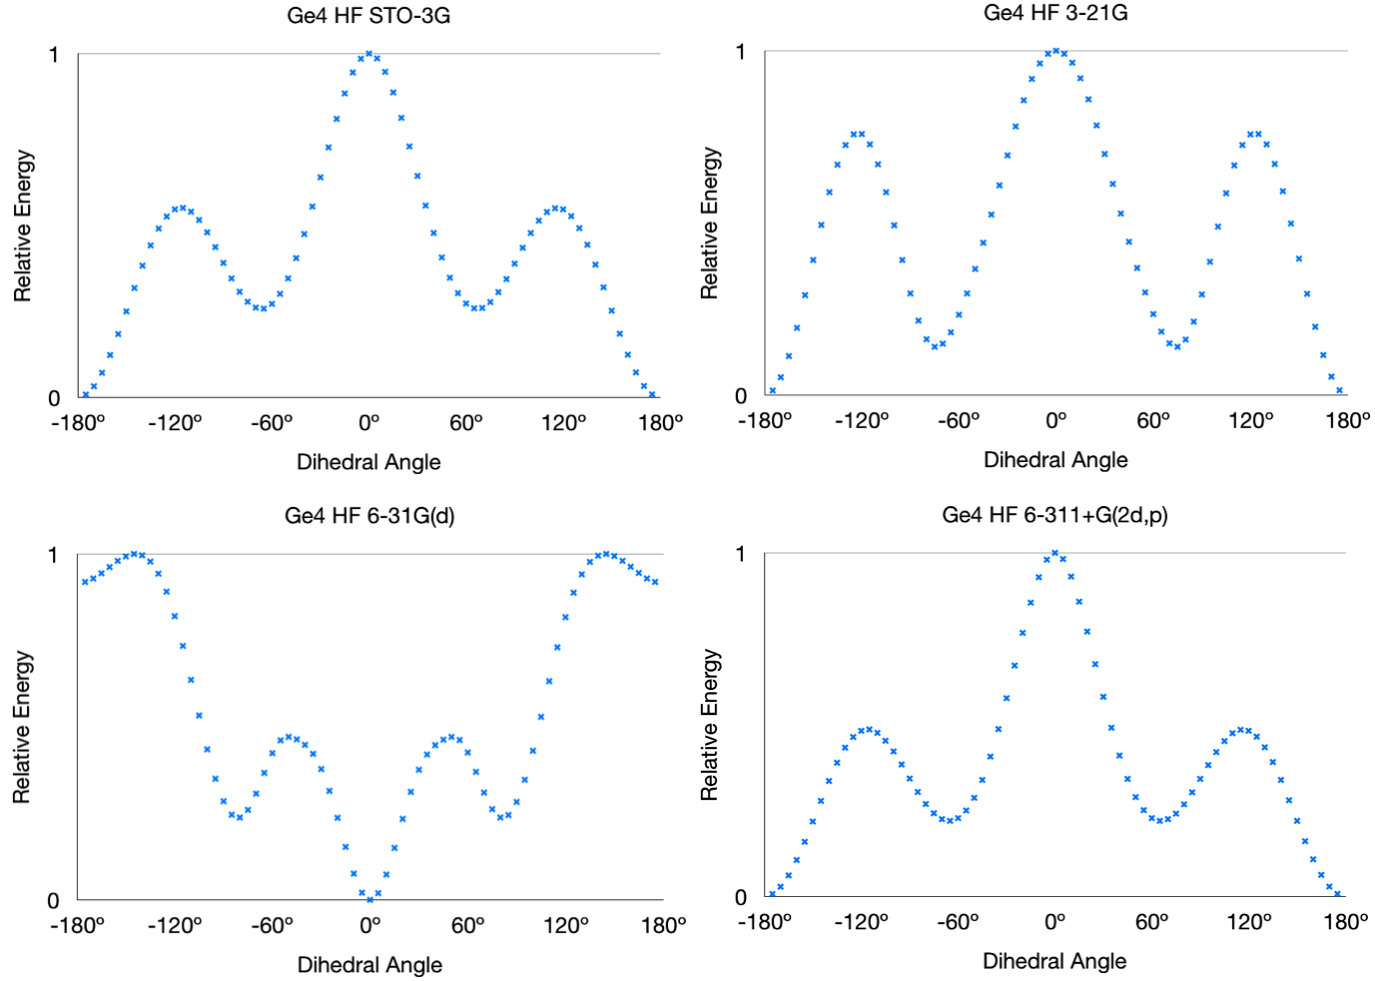
\includegraphics[width=\textwidth]{geTorsOne.png}
	
	\caption{Hartree Fock energy minimization of butagermane torsion run at varying basis sets.}
	
	\label{fig:geTorsOne}
	
\end{figure}

\begin{figure}
	
	\centering
	
	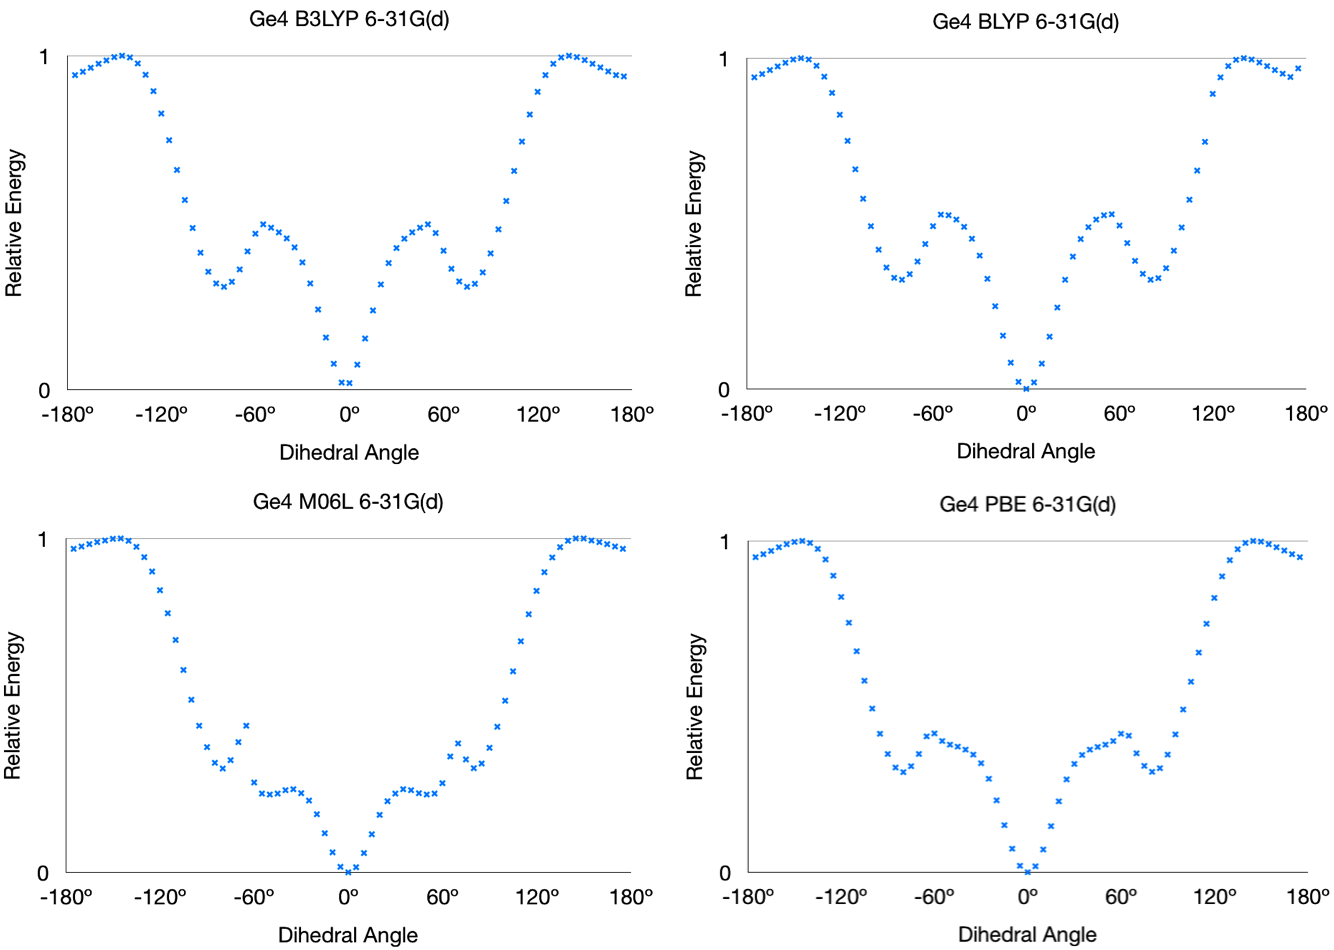
\includegraphics[width=\textwidth]{geTorsAll.png}
	
	\caption{Minimization of butagermane torsion run at varying theories and the 6-31G(d) basis set.}
	
	\label{fig:geTorsAll}
	
\end{figure}

\begin{figure}
	
	\centering
	
	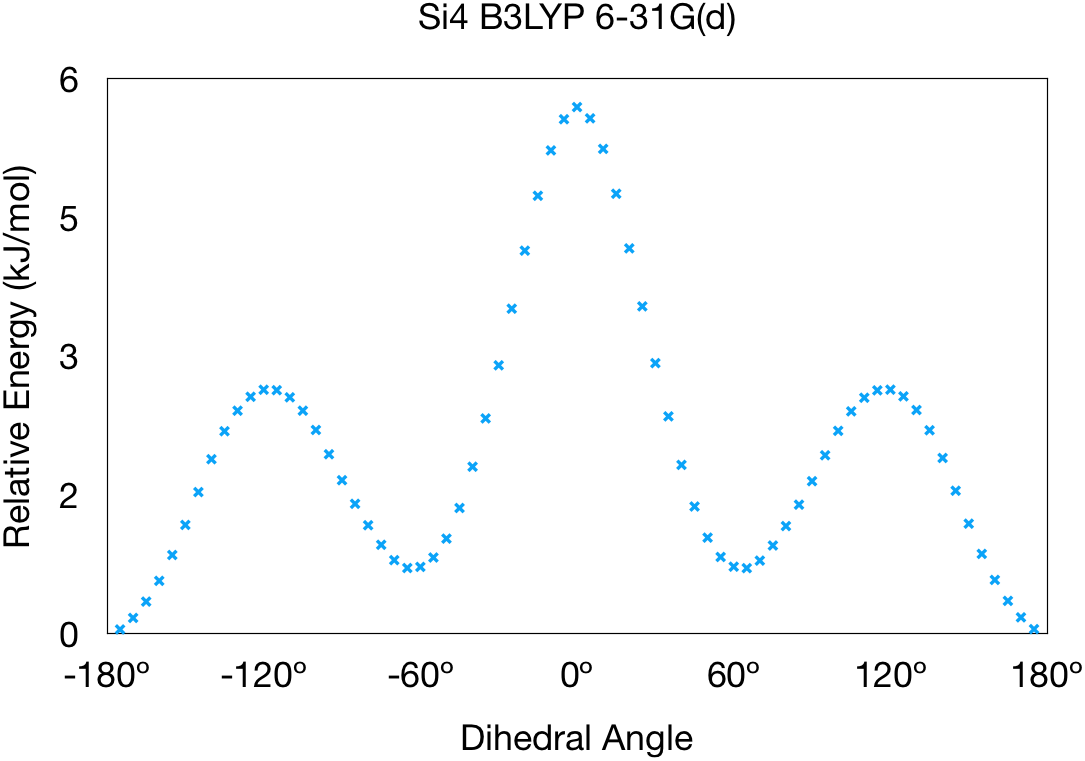
\includegraphics[width=0.75\textwidth]{siTorsOne.png}
	
	\caption{B3LYP energy minimization of butasilane torsion run at 6-31G(d) basis set.}
	
	\label{fig:siTorsOne}
	
\end{figure}


\begin{table}[]
	\centering
	\begin{tabular}{lllll}
		Program & \begin{tabular}[c]{@{}l@{}}Trans Energy\\ (Hartree)\end{tabular} & \begin{tabular}[c]{@{}l@{}}Cis Energy\\ (Hartree)\end{tabular} & \begin{tabular}[c]{@{}l@{}}∂ Energy\\ trans - cis\\ (Hartree)\end{tabular} & \begin{tabular}[c]{@{}l@{}}∂ Energy\\ trans - cis\\ (kcal / mol)\end{tabular} \\ \hline
		\multicolumn{1}{l|}{Gaussian} & -8298.8259 & -8298.8268 & -0.0009 & -0.5775 \\
		\multicolumn{1}{l|}{GAMESS} & -8306.1290 & -8306.1290 & 0.0040 & 2.4975 \\
		\multicolumn{1}{l|}{NWChem} & -8306.1290 & -8306.1250 & 0.0040 & 2.4974
	\end{tabular}
	\caption{Energy comparison of HF theory with 6-31G(d) basis set across multiple computational programs. The expected ∂E should be positive.}
	\label{tab:geHFAppData}
\end{table}

\section{Final Thoughts}

Unfortunately, a trend for simplifying the computation requirements of germanium was not discovered.
While it may exist among the data as a more involved function or as some other representation, there also may very well be no simple trend for switching between germanium and another group IV element.

On a much more interesting note, the results of the torsion drives revealed that Gaussian 03 and 09 contain some mistake within the 6-31G(d) basis set data for germanium. 
Considering the popularity of Gaussian software in computational chemistry, there are concerning implications about reliability of data for any germanium energy data with the 6-31G(d) basis set. 
Given that the torsion tests produced expected data for 6-31G(d) data subsequently run through a higher or lower basis set, only reported data with 6-31G(d) as the final calculated energy need be considered.
It is recommended that any investigator into computational aspects of germanium either replace the basis set data, use another basis set, or instead use a program like GAMESS or NWChem for that final computation.




\chapter{Sampling Conformation Landscapes by Rotatable Bond Degrees of Freedom}
\label{ch:ConformationLandscape}

\section{A Brief History on Conformation Landscapes}

\subsection{Levinthal's Paradox}

In 1969, a molecular biologist by the name of Cyrus Levinthal proposed a thought experiment regarding protein formation\cite{Levinthal}:

Consider a relatively small 150-residue peptide chain completely unfolded.
This protein will have 149 peptide bonds and therefore 149 phi angles and 149 psi angles. 
Assuming three possible angle positions each, the number of possible folds of this protein follows as $3^{298}$.
How does this peptide chain fold into the appropriate secondary and tertiary structures? 
Even at attosecond rates of rotating and folding, this peptide chain would likely not fold into the correct structure for many times the age of the universe!
Obviously, this is not the case, since proteins fold on the timescale of microseconds to milliseconds.\cite{LevParadoxCalculated}
How, then, do proteins fold so quickly and efficiently?
The answer lies in energy cascades through a visualization tool called a golf course.

\subsection{Levinthal Golf Courses}

If one imagines the energy landscape of a peptide chain like a golf course, interesting similarities arise.
For example, the lowest point could be considered ``the hole" of the course with the lowest energy conformer. 
When starting at the ``tee off" point, there may not be a clean pathway of energetic difference for the ball to roll toward the global minima.
Therefore, the ball must be ``struck" toward the hole in a series of motions where the ball is removed from one local minima and placed in another hopefully closer to the hole. 
Like the image shown in figure \ref{fig:DillGC}, the course is not always an easy, natural cascade toward the global minima.
Most often, investigators will initiate several searches in several locations of this conformation landscape in hopes that one will discover a clear minimum that is hopefully the true global minimum.

\begin{figure}
	
	\centering
	
	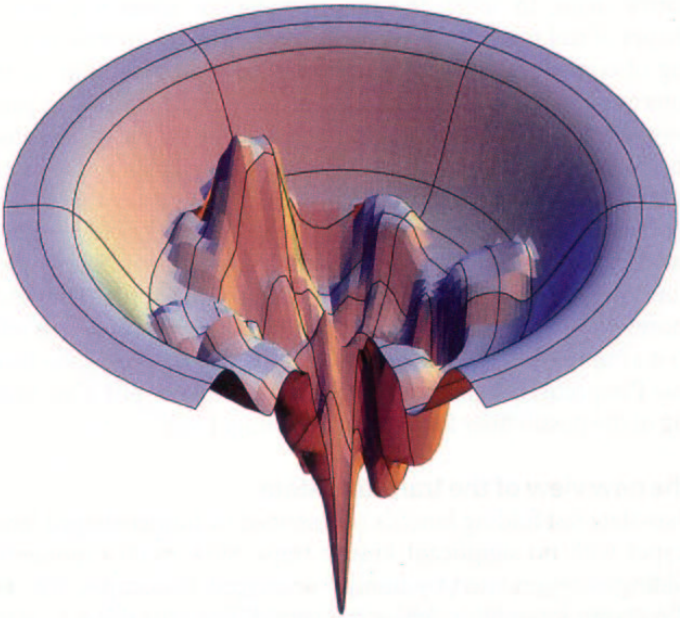
\includegraphics[width=0.75\textwidth]{DillGC.png}
	
	\caption{Example Levinthal Golf Course taken from Dill et al. \cite{DillLevGC}.}
	
	\label{fig:DillGC}
	
\end{figure}


\section{Purpose of Project}

As introduced in chapter \ref{ch:Germanium}, there may be a generic solution toward determining the lowest energy conformer by roughly sampling the full ``golf course" and procedurally focusing in on hot spots using automated methods.
Ideally, the tool would work through the seemingly infinite possibilities and quickly remove the impossible or duplicate conformers.
The tool would roughly take shape though a design flow detailed below.

First, the system takes an input molecule and generates a number of conformers based on rotatable dihedrals.
Second, a time-effective geometry optimization theory and basis set if necessary is selected and run files are generated and submitted to a cluster to compute.
Third, the results are collected and analyzed; low-energy dihedral values are passed back through the system while high-energy dihedrals are logged and discarded.
This restricts the conformation space to reduce the overall number of conformers generated and allows for more accurate and computationally-expensive theories and methods to calculate more reliable energies.

An overview of system flow given in figure \ref{fig:VRSDesign}.
\begin{figure}
	\centering 
	\makebox[\textwidth][c]{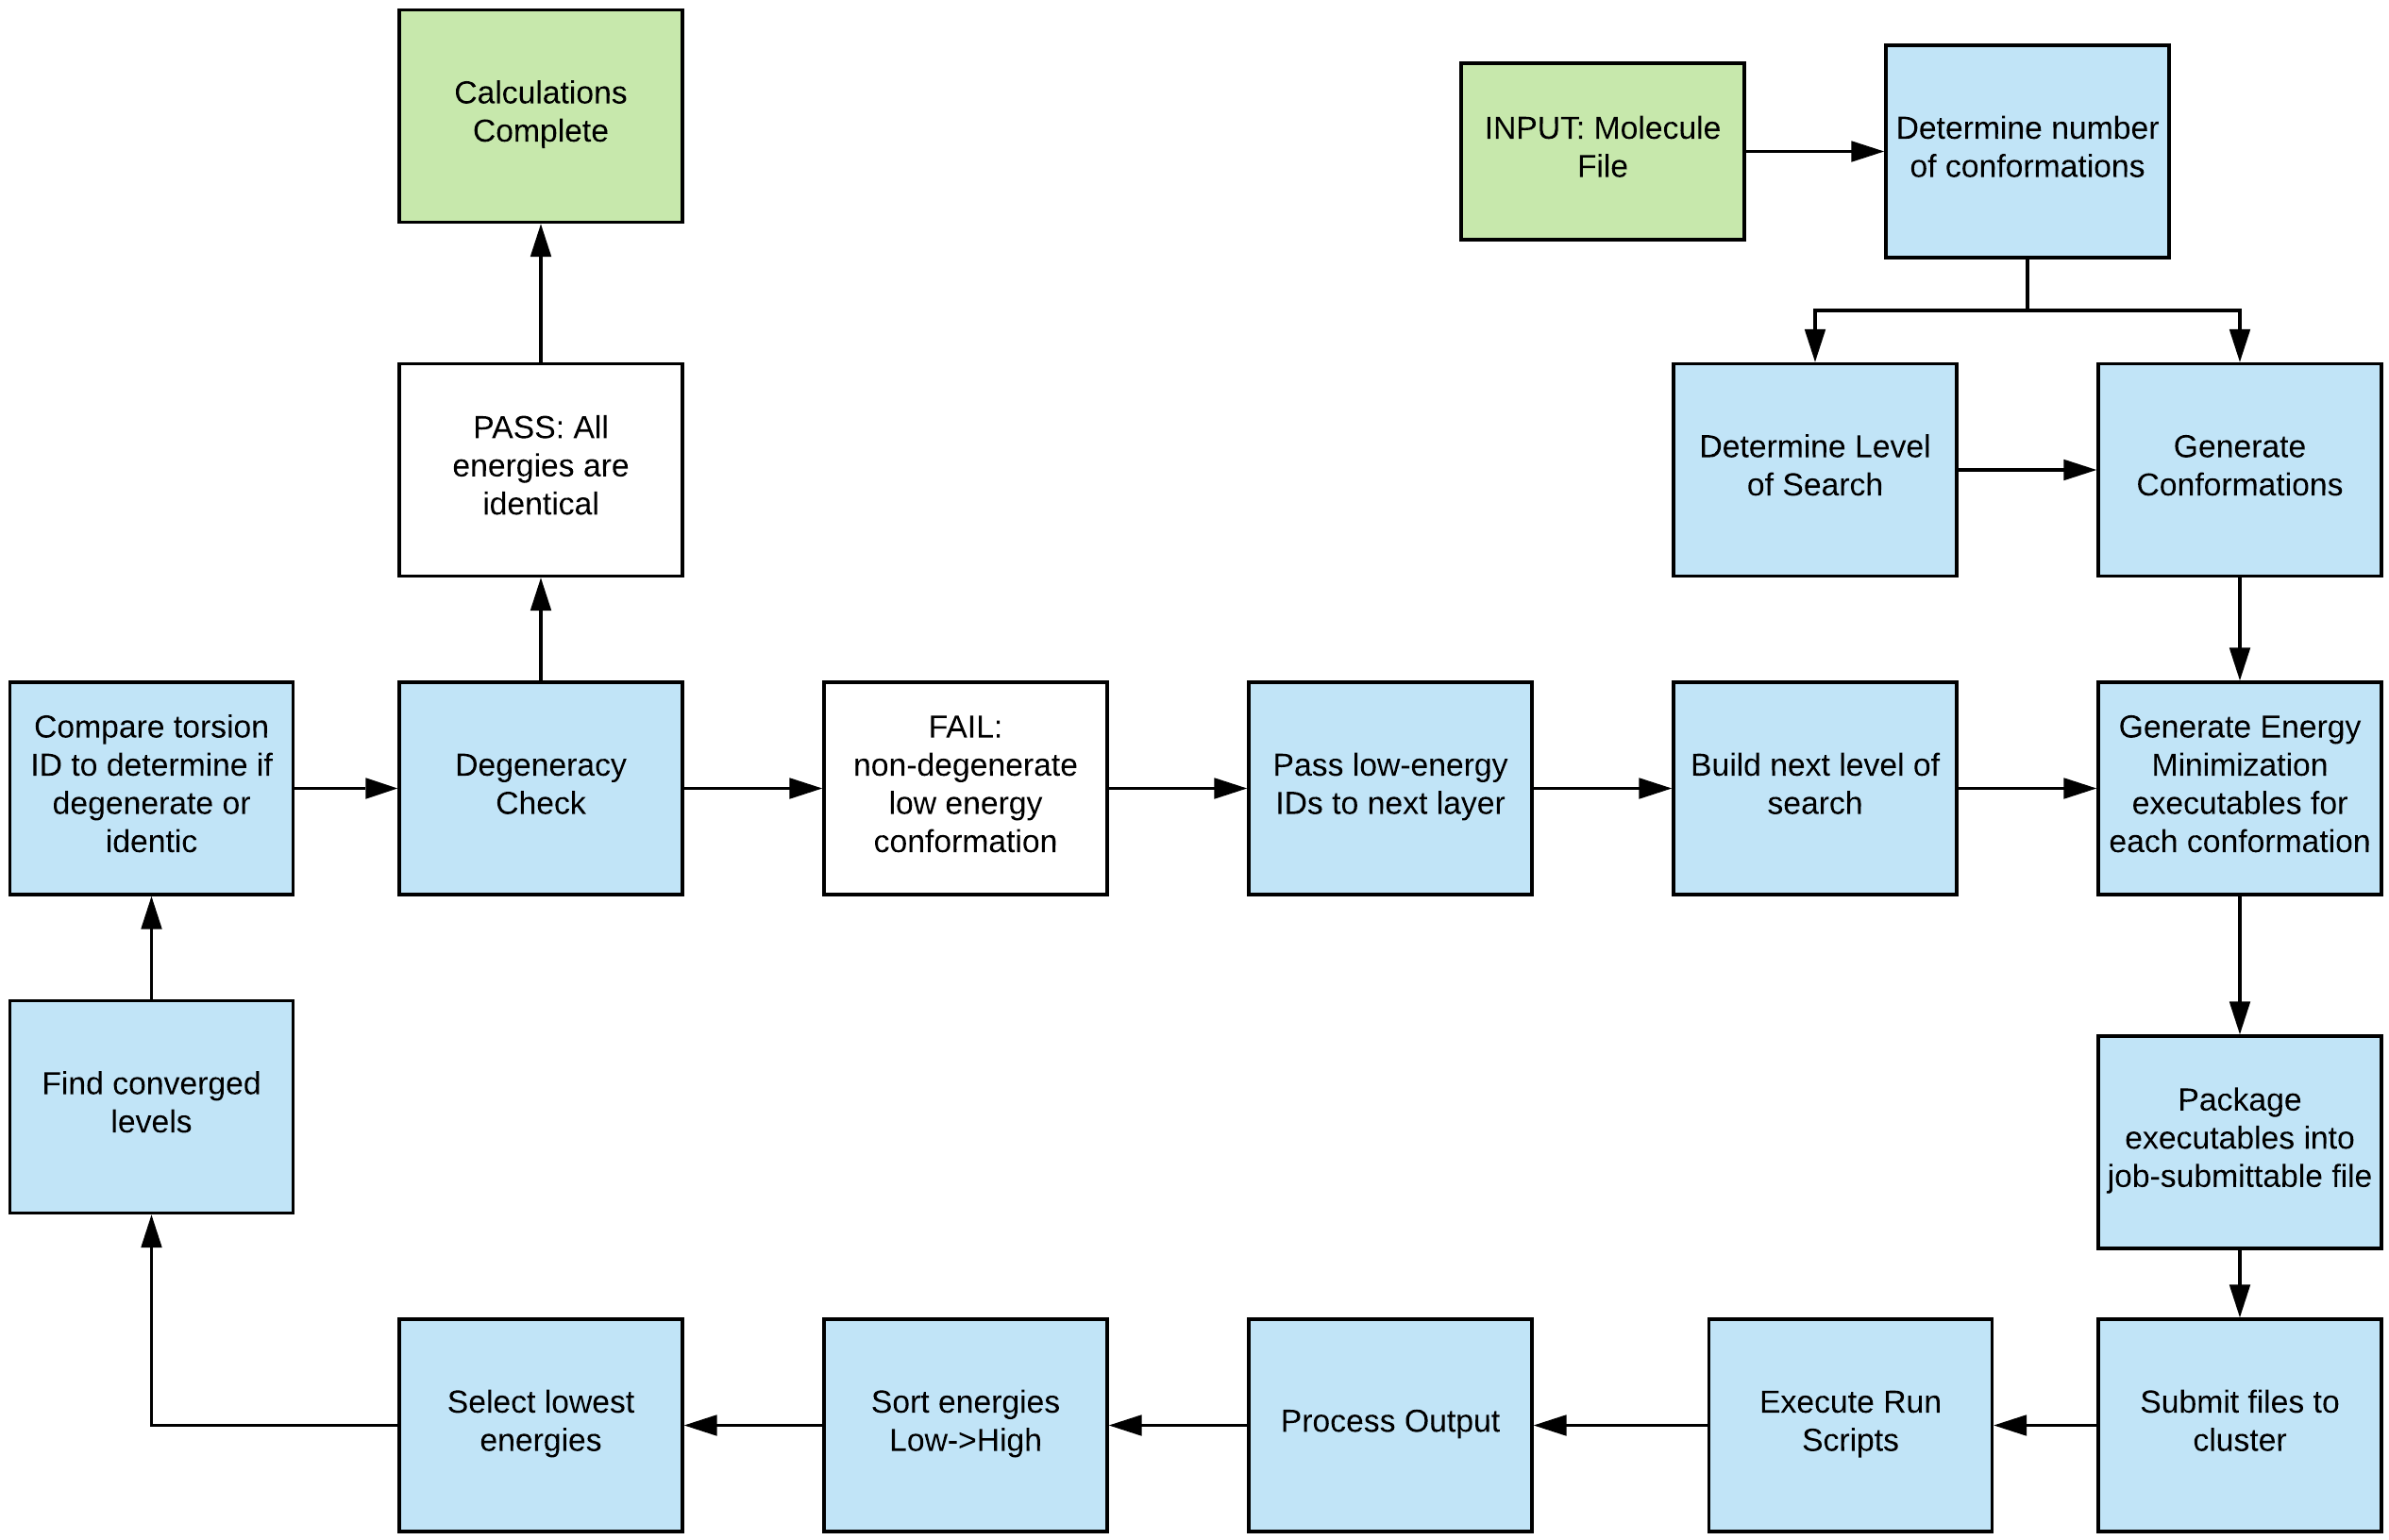
\includegraphics[width=1.3\textwidth]{AlgFlow.png}}
	\caption{Flow of method design for variable resolution conformation landscape search.}
	\label{fig:VRSDesign}
	
\end{figure}
This method produces an interesting multilayered visual plot with a zooming effect toward the lowest energy conformer.
An example of how this might look for a two-dihedral molecule is given in figure \ref{fig:variableResolutionSample}.
The outlined black boxes represent found regions of interest for future iterations of the method. 
This would repeat as necessary until regions converge to one energy.

\begin{figure}
	
	\centering
	
	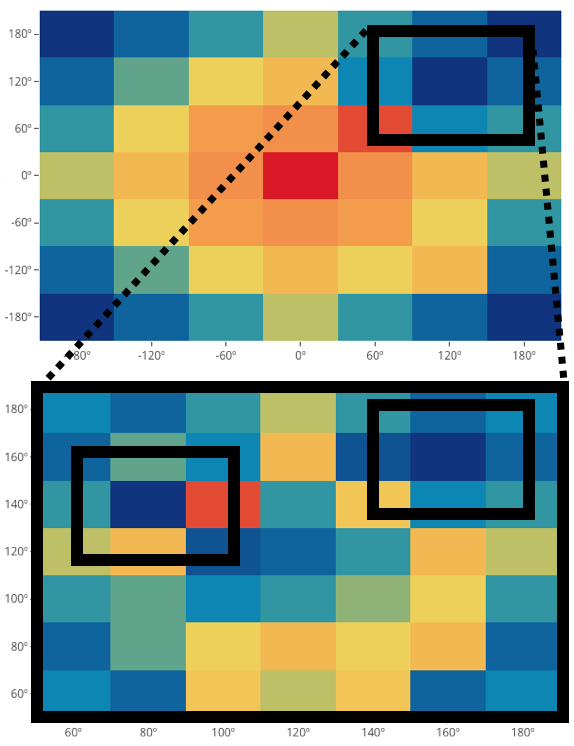
\includegraphics[width=0.75\textwidth]{VRSGraphEX.png}
	
	\caption{Example variable resolution search chart of two dihedrals with low-energy blue to high-energy red.}
	
	\label{fig:variableResolutionSample}
		
\end{figure}

\section{Design of System}

This system designed in Python for ease of development and compiled via Cython for computational efficiency. 
While it currently utilizes Gaussian 09 for energy minimization and UCSF Chimera for conformer generation, it can be redesigned for any computational programs that accomplish the desired tasks.

\subsection{Variation of Theory and Basis Set Usage by System Size and largest atom type}

Given that computational requirements increase with the number of atoms in a molecule and both the accuracy of the theory and basis set used, an initial focus on a manageable amount of conformers with a sufficiently simple theory and basis set is essential to success.
The system should estimate quantity and cost of calculations based on physcal computational constraints for various theory-basis set pairings. 
The system optimizes calculation types for the scope of the landscape.
Effectively, it balances between running the first broad-scope search at relatively low accuracy and a final near-final conformation space with relatively high accuracy methods.

% Good to have: data on how theory and basis set alter computational requirement. Available in literature? Create data from runs?

\subsection{Computational Optimization by Varying Resolution}

A common problem in all works on this topic is that the scale of truly searching the conformation landscape is expansive in even the most restrictive designs. 
The manual efforts in the design of this tool are to build checkers for impossible conformations, including overlapping atom spaces.
Additional considerations are that only the most bare, three conformations per rotatable bond angle, be considered initially.
After the first round of calculations, the scope of candidates should be reduced by several orders of magnitude by refining the search about lower energy regions in the landscape.


\subsection{Inherent Complications}

The single greatest complication of this and any energy landscape tool is the number of rotatable bonds in the target molecule and, to a lesser extent, the elements contained.
Consider the hexagermane molecule of interest in chapter \ref{ch:Germanium} and the general focus of this work.
One can focus on the number of torsions available to be adjusted in the energy landscape, as shown in figure \ref{fig:Ge6Torsions}. 
Even with the minimal three rotations per bond, these 19 rotatable bonds produce $3^{19} = 1,162,261,467$ conformers, which is realistically impossible to explore even with a computational method requiring five seconds to compute.
184 years of computation time would be required.
This is where the balance between recognizing impossible conformations comes in.
Especially with bulky molecules like this hexagermane, many conformations could be eliminated by way of checking for overlapping atoms.

\begin{figure}
	\centering 
	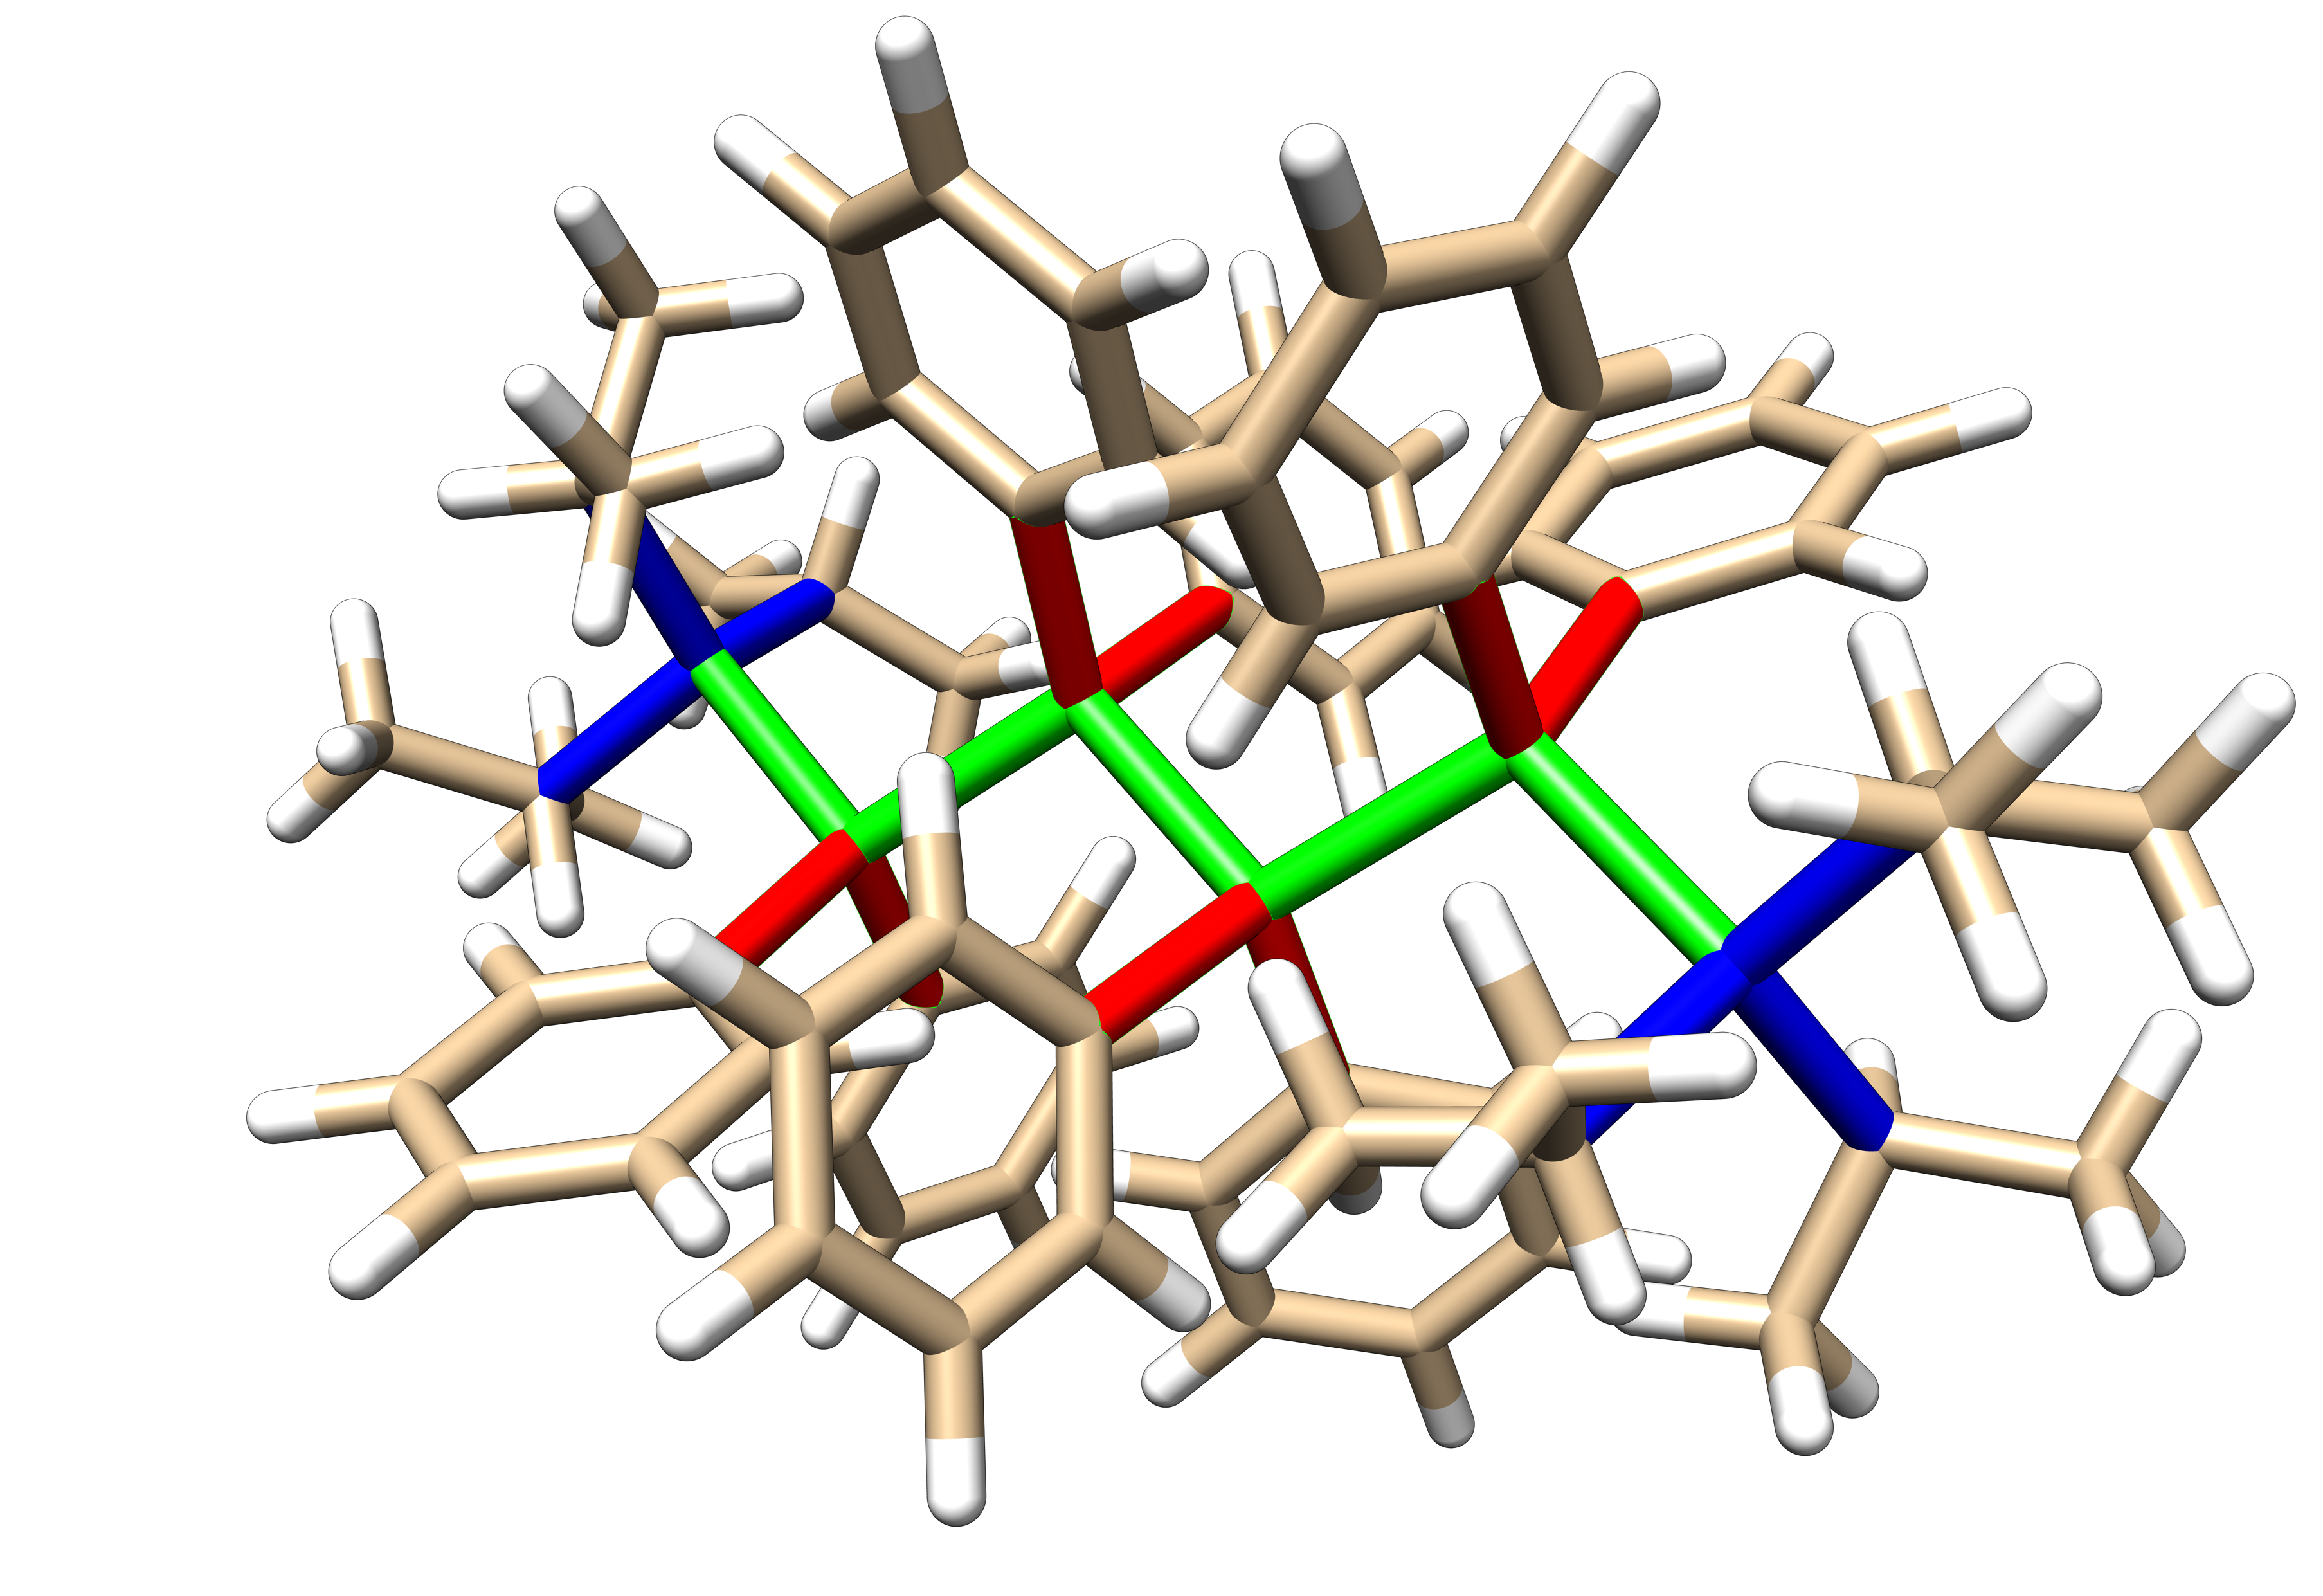
\includegraphics[width=0.75\textwidth]{Ge6Torsions.png}
	\caption{Highlighted torsions of the hexagermane molecule by type of bond, where green, red, and blue represent Ge-Ge, Ge-phenyl, and Ge-isopropyl torsion centers, respectively.}
	\label{fig:Ge6Torsions}
\end{figure}


\section{Results}

Due to the scale of the hexagermane molecule, a clear answer has not yet been discovered.
However, a much more simple run with o-nitrophenol, with only two rotatable bonds, was successful in finding the known highest and lowest energy conformer shown in figures \ref{fig:onpBad} and \ref{fig:onpGood}, respectively.

\begin{figure}
	\centering 
	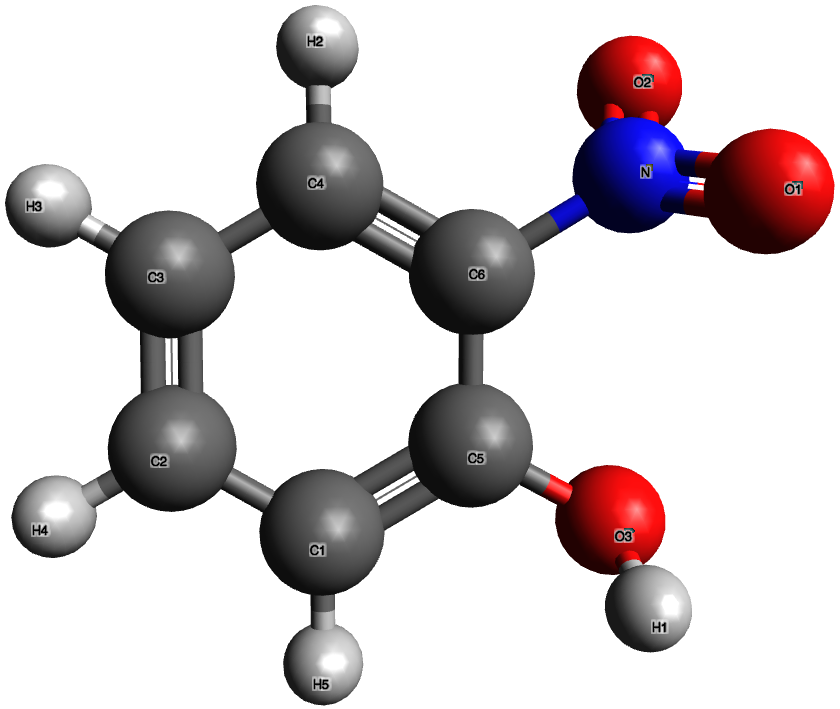
\includegraphics[width=0.75\textwidth]{onpBad.png}
	\caption{Highest energy conformer of o-nitrophenol, ignoring any ring strain conformations. This structure was notably unable to rotate and form the expected hydrogen bond between the ortho nitro and hydroxyl.}
	\label{fig:onpBad}
\end{figure}
\begin{figure}
	\centering 
	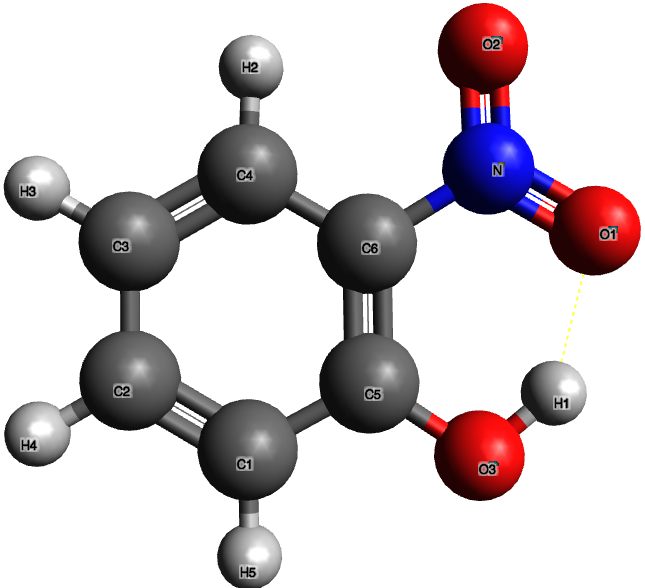
\includegraphics[width=0.75\textwidth]{onpGood.png}
	\caption{Lowest energy conformer of o-nitrophenol. Formed the expected hydrogen bond between the ortho nitro and hydroxyl.}
	\label{fig:onpGood}
\end{figure}

While these would have ideally been produced through a self-perpetuating system at increasing precisions and computation accuracy, the automated tool remains to be realized.

\subsection{Difficulties and Anticipated Future Approaches}

A key difficulty in automation of this tool is defining an abstract computation level based on arbitrary hardware limitations.
While currently limited to the Cowboy cluster at Oklahoma State University, the goal is that this tool be made available for chemists everywhere one day.
A potential solution for this abstract definition would be a small series of test runs to determine computational cost and general resource availability.

Additionally, the number of rotatable bonds yields the single largest barrier to searching the full conformation space.
With continued investigation and the inclusiveness with other works, it seems feasible that the insurmountable barrier to entry may yet be simplified in an objective way that does not prevent the system from finding the lowest energy conformer in any reasonably small molecule.

%\chapter{Conclusion}
\label{ch:Conclusion}

\section{Ice I$_{h}$ Generation}

Review:
\subsection{Purpose}
\subsection{Results}
\subsection{Flaws/Improvements}
\subsection{Practical Implications} 
Easier to generate crystals for modeling research

\section{Conformation Landscapes}

Review:
\subsection{Purpose}
\subsection{Results}
\subsection{Flaws/Improvements}
\subsection{Practical Implications} 
Collected Program for general use

\section{Modeling Germanium Compounds}

Review:
\subsection{Purpose}
\subsection{Results}
\subsection{Flaws/Improvements}
\subsection{Practical Implications} 
Discovered mistake to be fixed

\section{Two-Dimensional Water}

Review:
\subsection{Purpose}
\subsection{Results}
\subsection{Flaws/Improvements}
\subsection{Practical Implications} 
super-duper anti-freeze? also freezing point elevation.

\section{Super Duper Final Conclusion}



%===================== bibliography ============================================
%\nocite{*} %leave this to put ALL references in the bibliography
\newpage
\renewcommand\bibname{References}
\addcontentsline{toc}{chapter}{References}
\bibliography{References/References} %use main dissertation bibtex file
\bibliographystyle{agsm}

%====================== appendices ==============================================
\appendix
\singlespace
\chapter{Ice Ih to Ice XI Conversion}
\label{ch:App:CrystalDisorg}

Listed below is the source code utilized in the conversion of a PDB Ice Ih structure into an Ice XI structure. This code is functional in a Python 2.7 environment with NumPy and SciPy packages included.

\section{Code: Crystal Disorganizer Tool}
\lstinputlisting[language=Python,breaklines=true]{codes/PDBDisorganize.py}


\chapter{Two-Dimensional Rose-Potential Water}
\label{ch:App:2DWater}

Below is the python script used to adjust the Rose-Potential system for various interfaces.

\section{Code: Surface Adjustment Tool}
This tool was created to adjust surface information in a given system.
\lstinputlisting[language=Python,breaklines=true]{codes/oopseSurfaceMaker.py}

% This is monstrous - unreasonable to include
% \section{Surface Visualization Tool}
% This tool was provided by Dr. Fennell to convert the completed OOPSE run into povre files to be converted into images or gifs.
% \lstinputlisting[language=Perl,breaklines=true]{codes/surfaceRose2pov.pl}


\chapter{Germanium Landscape}
\label{ch:App:Germane}

\section{Sample Gaussian 09 Germanium File}
\label{SampleGeRunFile}
Command files like the one below were built using Dr. Fennell's Gaussian 09 run builder script and proved very effective in producing command files.
\lstinputlisting[breaklines=true]{codes/6geSample.cmd}

\section{Building Group 4 Chains}

While briefly mentioned and the subject of research for some time, the butyl-IV chain builder is detailed below. 
Ultimately unsuccessful in the initial trials, these scripts may serve a purpose in further work.

This first script builds a parent set of all possible C, Si, and Ge butylalkyl chains.

\lstinputlisting[language=Python,breaklines=true]{codes/grp4builder.py}

This second script takes the original trans-all butyl chain and enumerates 72 torsional rotations into a folder.

\lstinputlisting[language=Python,breaklines=true]{codes/ChimeraRot.py}

\section{Collecting and Comparing Torsional Data}

These two scripts were utilized to reduce the output data into an energy value with normalized intensity from 0 to 1. The third script compares two of these files and looks for any additive or multiplicative trend.

This first file reads energy data and creates a list of absolute energy values per torsion degree.
\lstinputlisting[language=Python,breaklines=true]{codes/4gepullStatPDBs.py}

This second file converts the first file into a relative scale from 0 to 1.
\lstinputlisting[language=Python,breaklines=true]{codes/4getreatAbsEnergies.py}

This third script compares two generated files using the prior scripts. It can compare the generated absolute energy with the relative energy files. It was often run as a loop through every permutation of the group 4 builder.

\lstinputlisting[language=Python,breaklines=true]{codes/compEnerData.py}


\chapter{Conformation Landscapes}
\label{ch:App:ConfLand}

Listed below are two example Germanium PDB files. The first is for the end-goal hexagermane in the trans-trans-trans conformation with isopropyl groups on the terminal Ge atoms. The second is for the simplified butagermane with fully protonated Germanium atoms.

\section{Code: hexagermane-transall.pdb}

\lstinputlisting[breaklines=true]{codes/hexagermane-transall.pdb}

The above molecule contains 154 atoms and 153 bonds, making it extremely computationally expensive for regular QM calculations. This made utilizing the large molecule as a trial system unreasonable due to the prohibitively long computation time for each conformation, assuming the conformation calculation would complete at all.

The below PDB file is the simplified butagermane with fully protonated Germanium atoms. As a significantly smaller system with only 14 atoms and 13 bonds, the relatively short computation time allowed the trial system to move with relative ease.

\section{Code: ge4h.pdb}

\lstinputlisting[breaklines=true]{codes/ge4h.pdb}

\section{Progress on Torsion Minimizer System}

While incomplete and largely nonfunctioning, this code is the current progress toward the implementation of the torsion minimizer system as outlined in \ref{fig:VRSDesign}.

\lstinputlisting[language=Python,breaklines=true]{codes/DTM/Runner.py}


%====================== vita ====================================================
\newpage
\begin{vita}{Gentry H. Smith}{Master of Science}{Chemistry} %Creates vita
    \vitaitem{Personal Data:} Born in Olathe, KS in November 1993.
    \vitaitem{Education:} \\ Received a Bachelors of Science in Chemistry at Southern Nazarene University in May 2016. \\ \\
Completed the requirements for the degree of Master of Science with a major in Chemistry at Oklahoma State University in May 2018.
    \vitaitem{Experience:} \\ 
    \vitaitem{Professional Affiliations:} \\ American Chemical Society
    \vitaitem{Awards}\\ Colonel Andre Whitely Scholarship in Chemistry
\end{vita}


\end{document}
